\documentclass[11pt,letterpaper]{article}
\usepackage[
  letterpaper,
  top=0.75in,
  bottom=0.75in,
  left=0.75in,
  right=0.75in,
  headheight=14pt,
  headsep=12pt,
  footskip=18pt
]{geometry}

\usepackage{fontspec}
\setmainfont{Helvetica}
\setmonofont{Menlo}

\usepackage{amsmath,amssymb,amsfonts}
\usepackage{booktabs}
\usepackage{tabularx}
\usepackage{graphicx}
\usepackage{xcolor}
\usepackage{hyperref}
\usepackage{caption}
\usepackage{microtype}

\hypersetup{
  breaklinks=true,
  colorlinks=true,
  linkcolor=blue!70!black,
  citecolor=blue!70!black,
  urlcolor=blue!70!black
}

\def\UrlBreaks{\do\/\do\a\do\b\do\c\do\d\do\e\do\f\do\0\do\1\do\2\do\3\do\4\do\5\do\6\do\7\do\8\do\9\do\-}

\captionsetup{font={small},labelfont={bf},skip=6pt}

\title{\textbf{Multi-Trial Reliability and Failure Concentration in Multi-Hop AI Agents}\\[0.3em]\large Grounding Collapse, Failure Taxonomy, and Evaluator Calibration}
\author{
  \textbf{Samir Sawarkar}\\
  FAULTLINE AI Reliability Engineering\\
  \texttt{samir@faultline.ai}\\
  \url{https://github.com/samirsawarkar/faultline-ai-reliability}
}
\date{September 2026}

\begin{document}
\sloppy
\maketitle

\begin{abstract}
When deploying autonomous language model agents on critical multi-step tasks, system architects require joint operational reliability across repeated runs [12, 23]. In evaluation practice, a common working assumption is that the multi-trial success rate $\text{pass}^k$—the probability that an agent completes all $k$ independent repetitions of a task—can be estimated by extrapolating single-trial benchmark accuracy via the naive independent Bernoulli formula $\text{pass}^k = (\text{pass@1})^k$. While $\tau$-bench reports $\text{pass}^k$, it does not benchmark the empirical gap to $(\text{pass@1})^k$; in this work, we test this gap directly on a controlled, contamination-resistant 5-hop knowledge retrieval benchmark with 150 held-out hard scenarios executed over $k=3$ repeated trials graded by a deterministic dual-condition oracle without subjective model judges in the loop. We report the pre-registered \emph{as-run} analysis ($n=150$) alongside an \emph{infra-excluded} sensitivity analysis ($n=117$) that purges external cloud gateway dropouts. Our pre-registered working hypotheses H4 (that measured $\text{pass}^3$ strictly exceeds naive $(\text{pass@1})^3$) and H5 (that positive deviation from naive compounding is larger on cheaper model tiers) are both \textbf{NOT\_TESTABLE\_AS\_PREREGISTERED} because only 2 of 6 rungs produced valid data; on the valid rungs, R4 met the pre-registered per-rung criterion under both as-run and infra-excluded variants while R2 did not. Crucially, across both evaluated commercial model tiers, naive Bernoulli compounding matches empirical observations within 2.5 percentage points at $k=3$, predicting joint reliability within 2.5 percentage points of measured values—well within our pre-registered 10 percentage point minimum effect of interest. For the higher-accuracy tier (R2, $\text{pass@1} = 0.6311$), repeated outcomes are consistent with a homogeneous-binomial null ($\text{pass}^3 = 0.2267$ vs naive $0.2514$, parametric bootstrap goodness-of-fit $p = 0.3794$, Tarone overdispersion $z = -0.655, p = 0.7438$, $\text{ICC}(1,1) = -0.0287$, $C_3 \in [0.7161, 1.0793]$). For the lower-accuracy tier (R4, $\text{pass@1} = 0.1489$ as-run), an apparent excess of 3-of-3 successes ($\text{pass}^3 = 0.0200$ vs naive $0.0033$, parametric bootstrap $p = 0.0053$) is heavily driven by serving infrastructure dropouts. Purging dropouts ($n=117$) leaves only a marginal excess ($\text{pass}^3 = 0.0256$ vs naive $0.0070$, exact tail $p = 0.0488$, Tarone $z = 0.764, p = 0.2224$), rendering the concentration ratio $C_3$ unresolved with a 95\% bootstrap confidence interval of $[0.0000, 7.5772]$ spanning 1.0. While observations at $k=3$ cannot separate across-scenario heterogeneity from within-scenario serial dependence, beta-binomial compounding extrapolation demonstrates that even undetectable intra-scenario correlation ($\text{ICC}_{\text{hi}} = 0.0668$ on R2) yields compounding divergence at larger depths ($C_8 \approx 2.25$, $\text{pass}^8 \approx 0.057$ vs naive $0.025$). All runs were conducted at pinned temperature 0.0, where run-to-run variation is driven by serving infrastructure nondeterminism rather than stochastic sampling [10, 16, 18].
\end{abstract}


\section{Introduction}

For LLM tool-use agents on a fixed set of 5-hop grounded-retrieval tasks, does the joint reliability over $k$ repeated executions equal the independence prediction $\text{pass}^k = (\text{pass@1})^k$, and if not, in which direction and by how much? Autonomous language model agents are increasingly integrated into operational pipelines where single-turn success is insufficient [1, 23]. Deployments require execution stability across repeated invocations on the same task instance [12, 23]. In standard evaluation, $\text{pass@k}$ was formalized by Chen et al. [2] as an unbiased estimator for whether at least one of $k$ generated code samples succeeds. In contrast, autonomous agent reliability requires joint consistency: $\text{pass}^k$, defined by Yao et al. [23] as the probability of successfully completing all $k$ repeated interaction episodes on a task instance.

In engineering practice, a common working assumption is that single-run evaluation scores ($\text{pass@1}$) can be extrapolated to predict multi-execution reliability by assuming repeated runs behave as independent Bernoulli trials: $\text{pass}^k = (\text{pass@1})^k$. This assumption presumes that task difficulty is homogeneous and that repeated executions fail independently. When agents encounter structural obstacles, such as search loops or query syntax errors, failures can concentrate within specific scenario instances. Under across-scenario heterogeneity, tractable tasks pass reliably while intractable tasks fail, causing measured $\text{pass}^k$ to exceed $(\text{pass@1})^k$ via Jensen's inequality. Conversely, if execution paths diverge unpredictably due to serving engine jitter, runs may compound independently [10, 18].

Existing agent benchmarks typically publish point estimates of $\text{pass@1}$ without instance-level confidence intervals or formal tests of independence [15]. Additionally, evaluations often rely on subjective LLM judges that introduce position, verbosity, and self-enhancement biases [17, 25].

We present a controlled empirical test of the independence assumption $\text{pass}^k = (\text{pass@1})^k$ on a synthetic, contamination-resistant 5-hop knowledge graph benchmark. We execute 150 held-out hard Tier-3 scenarios across $k=3$ repetitions under greedy decoding (temperature 0.0) across two commercial model tiers: a fast tier (R2: \texttt{z-ai/glm-5.3-flash}) and a frontier tier (R4: \texttt{openai/gpt-5.6-luna}). We grade every trial with a deterministic dual-condition oracle requiring exact answer normalization and verified document citation, eliminating model judges from the evaluation loop. We treat the comparison between R2 and R4 strictly as evidence regarding different accuracy regimes under repetition rather than a general capability ranking.

Our contributions are:
1. \textbf{Empirical test of the independence assumption:} We provide a formal statistical test of $\text{pass}^k = (\text{pass@1})^k$ on 150 controlled multi-hop retrieval scenarios across two accuracy regimes ($k=3$). Across both models, the naive independent formula predicts joint reliability within 2.5 percentage points of measured values ($\Delta_3 = -0.0247$ on R2; $\Delta_3 = +0.0187$ on R4 infra-excluded), well below the 10 percentage point minimum effect of interest.
2. \textbf{Characterization of failure clustering and overdispersion:} We show that for R2 ($\text{pass@1} = 0.6311$), repeated execution outcomes are consistent with a homogeneous-binomial null ($C_3 = 0.9017$ [95\% CI $0.7161, 1.0793$], parametric bootstrap $p = 0.3794$, Tarone overdispersion $z = -0.655, p = 0.7438$, $\text{ICC}(1,1) = -0.0287$). For R4 ($\text{pass@1} = 0.1489$), an apparent excess of 3-of-3 successes is heavily driven by serving timeouts; purging dropouts leaves only a marginal 1.86 pp excess ($p_{\text{param}} = 0.0243$, Tarone $z = 0.764, p = 0.2224$), leaving $C_3$ unresolved with a bootstrap CI spanning 1.0 ($[0.0000, 7.5772]$).
3. \textbf{Compounding extrapolation and harness post-mortem:} We demonstrate via beta-binomial modeling that while $k=3$ cannot separate across-scenario heterogeneity from within-scenario serial correlation and leaves naive compounding accurate to 2.5 pp, even undetectable intra-scenario correlation ($\text{ICC}_{\text{hi}} = 0.0668$) compounds into notable divergence at scale ($C_8 \approx 2.25$, $\text{pass}^8 \approx 0.057$ vs naive $0.025$). Furthermore, our trace post-mortem demonstrates how external provider outages interact with client-side circuit breakers to fabricate false clustering signatures, and we quantify the two-pass execution where 18.9M tokens (34.8\%) were discarded.

\section{Question and Pre-Registration}

\subsection{Research Question}
We investigate the pre-registered research question:
\begin{quote}
\emph{For LLM tool-use agents on a fixed set of 5-hop grounded-retrieval tasks, does the joint reliability over $k$ repeated executions equal the independence prediction $\text{pass}^k = (\text{pass@1})^k$, and if not, in which direction and by how much?}
\end{quote}

The unit of analysis is the scenario instance ($n=150$ Tier-3 scenarios, IDs \texttt{r-0201} to \texttt{r-0350}). The $k=3$ executions per scenario represent repeated nested measurements; scenarios are the sampling units for all confidence intervals, bootstraps, and paired tests.

\subsection{Pre-Registered Hypotheses and Both-Outcomes Commitment}
Before data collection on Project P06, two primary hypotheses were pre-registered in \texttt{HYPOTHESES.md} (and \texttt{research/method/hypothesis.md}):
- \textbf{Hypothesis H4 (verbatim):} \emph{"Measured $\text{pass}^{3}$ strictly exceeds naive $(\text{pass@1})^{3}$ for $\ge$ 4 of 6 rungs."}  
  - \emph{Prediction if true:} 95\% Wilson score interval of measured $\text{pass}^3$ strictly excludes and exceeds naive $(\text{pass@1})^3$ on $\ge 4$ rungs.
  - \emph{Prediction if false:} Wilson interval of measured $\text{pass}^3$ contains or falls below naive on $\ge 3$ rungs.
- \textbf{Hypothesis H5 (verbatim):} \emph{"Deviation from naive compounding (delta = $\text{pass}^{3}$ - $(\text{pass@1})^{3}$) is larger for cheaper rungs than frontier rungs."}  
  - \emph{Prediction if true:} $\Delta_{R2} > \Delta_{R4}$; concentration ratio $C_3$ higher on R2 than R4.
  - \emph{Prediction if false:} $\Delta_{R2} \le \Delta_{R4}$ or rank ordering across the ladder is reversed.

The pre-registration committed to publishing findings regardless of outcome. Both H4 and H5 are \textbf{NOT\_TESTABLE\_AS\_PREREGISTERED} because only 2 of 6 rungs produced valid data (R6 was invalidated by gateway dropouts, and R1/R3/R5 remained unexecuted); on the 2 evaluable rungs, the per-rung criterion was met on R4 under both as-run and infra-excluded variants, and not met on R2.

\subsection{Frozen Artifact Hashes}
Pipeline artifacts were cryptographically pinned prior to execution:
- \textbf{Synthetic graph corpus:} \texttt{build\_corpus(42)}, SHA256 \nolinkurl{84e6ff590704aa94d10912f8002716b14c7436080e1a3270b53f9385dc728efc}.
- \textbf{Scenario manifest:} 150 Tier-3 scenarios (\texttt{r-0201}–\texttt{r-0350}), manifest SHA256 \nolinkurl{7e0a1b79d6e756f712d27e29168fed8b3bc5c4cd7beba7f8fc21d50366d41b83}.
- \textbf{System prompt:} \texttt{faultline\_p2/agent/prompt.py} (Amendment A-001), SHA256 \nolinkurl{87c7641e74964dcfe00c605051d7f5ddfade01f4019c95a00fd5dc3f1907c8df}.
- \textbf{Trace database:} \texttt{projects/p06\_passk/trace.db}, SHA256 \nolinkurl{1c83d147b5d7e5509a97eb46bf6fc400ca45b36aaa189bb18810bc75c56fe222}.



\section{Environment}

\subsection{Synthetic Pseudoword Knowledge Graph}
Real-world corpora suffer from pre-training contamination, enabling models to recall memorized facts [2]. To ensure contamination resistance, we construct a synthetic knowledge graph of 300 entities interconnected by directed relational edges, generated with master seed 42. All entity names, document IDs, relational predicates, and target attributes are coined pseudowords absent from public text. Documents define local attributes and outgoing relational pointers. Traversing the graph requires sequential tool calls: retrieving document $A$, extracting entity $B$, querying document $B$, and repeating until reaching terminal document $E$.

\subsection{Tier-3 Multi-Hop Scenarios}
The benchmark partitions tasks into three complexity tiers: Tier 1 (1-hop), Tier 2 (2–3 hops), and Tier 3 (5 hops). We isolate the reserved hard pool of 150 Tier-3 scenarios (\texttt{r-0201} to \texttt{r-0350}), requiring five sequential document traversals to locate the target attribute. This pool is unsaturated (pass rates range from 14.9\% on R4 to 63.1\% on R2 across the two valid rungs), preventing ceiling and floor saturation from masking trial variance [C009, C014].

\subsection{Deterministic Dual-Condition Oracle}
To eliminate automated judge biases [17, 25], we implement a deterministic dual-condition oracle (\texttt{faultline\_p2/oracle/oracle\_check}). An execution trial is scored as a success ($y_{i,j} = 1$) if and only if:
1. \textbf{Normalized Answer Match:} The final answer string, after lowercase conversion and punctuation stripping, matches the ground-truth terminal attribute.
2. \textbf{Cited Source Provenance:} The ground-truth document identifier containing the terminal attribute appears within the agent's citation list.

Hallucinated answers without citations, or retrieved documents without correct attribute extraction, are scored as failures ($y_{i,j} = 0$).



\section{Method}

\subsection{Protocol and Temperature Disclosures}
Each scenario $i \in \{1, \dots, 150\}$ is executed across $k=3$ distinct runs per model tier (450 trials per model, 1,350 total) with a 24-step cap (Amendment A-003, MEC v1.3) using \texttt{get\_document(doc\_id)} and \texttt{search\_entity(query)}. Each step constitutes one agent turn (model inference followed by tool execution); we score step-cap exhaustion without an oracle-verified answer as an incomplete failure. A single execution worker dispatched trials sequentially, looping over scenarios and repetitions with inter-trial pacing set by gateway response turnaround to prevent client-side concurrency contention.

All queries were executed with greedy decoding pinned to \texttt{temperature = 0.0}, \texttt{top\_p = null}, and \texttt{max\_tokens = 2048}. In benchmark literature, temperature 0 is assumed to ensure deterministic execution [10]. However, parallel GPU reduction kernels violate floating-point associativity: dynamic batching, concurrent thread scheduling, and kernel implementations alter summation order, inducing output divergence even at temperature 0 [8, 9, 10, 16, 18, 24]. When candidate token probabilities are close (particularly in the range 0.1 to 0.9), small numerical variations in logits can invert greedy argmax selection [8]. Thus, we interpret between-trial variation across our runs as inference engine and serving backend nondeterminism rather than stochastic sampling.

\subsection{Metrics: $\text{Pass@k}$ versus $\text{Pass}^{k}$}
Let $N = 150$ and let $y_{i,j} \in \{0, 1\}$ denote the binary oracle verdict for scenario $i$ on trial $j \in \{1, \dots, k\}$ ($k=3$). Single-trial accuracy is $\text{pass@1} = \frac{1}{N \cdot k} \sum_{i=1}^N \sum_{j=1}^k y_{i,j}$.

Chen et al. [2] defined $\text{pass@k}$ as the probability that at least one of $k$ generated samples succeeds among $n \ge k$ attempts ($c_i$ correct):
$$\text{pass@k} = \mathbb{E}\left[ 1 - \frac{\binom{n - c_i}{k}}{\binom{n}{k}} \right]$$
where $c_i = \sum_{j=1}^k y_{i,j}$; when $n = k$, this reduces directly to the probability of at least one success $\mathbb{I}(c_i \ge 1)$. For autonomous agents, Yao et al. [23] defined joint reliability $\text{pass}^k$ as the probability that all $k$ repeated interaction episodes succeed:
$$\text{pass}^k = \frac{1}{N} \sum_{i=1}^N \prod_{j=1}^k y_{i,j} = \frac{1}{N} \sum_{i=1}^N \mathbb{I}(c_i = k)$$

Under independent Bernoulli trials with parameter $p = \text{pass@1}$, expected joint reliability is $\text{naive } (\text{pass@1})^k = (\text{pass@1})^k$. We define the concentration ratio $C_k$ and deviation delta $\Delta_k$:
$$C_k = \frac{\text{pass}^k}{(\text{pass@1})^k}, \quad \Delta_k = \text{pass}^k - (\text{pass@1})^k$$
$C_k > 1.0$ ($\Delta_k > 0$) indicates positive failure concentration, $C_k = 1.0$ indicates perfect independence, and $C_k < 1.0$ indicates negative clustering.

\subsection{Statistical Testing Framework}
1. \textbf{Wilson Score Intervals:} Proportions report 95\% Wilson score intervals [22].
2. \textbf{Scenario-Level Percentile Bootstrap:} To account for nested trials, we compute confidence intervals for $\text{pass@1}$, $\text{pass}^k$, risk differences, and ratio $C_k$ using a scenario-level percentile bootstrap with 10,000 resamples (seed 42), resampling entire scenario vectors $(y_{i,1}, \dots, y_{i,k})$ [6].
3. \textbf{Parametric Bootstrap Goodness-of-Fit:} Under independence, $c_i \sim \text{Binomial}(3, \text{pass@1})$. Because single-trial accuracy $p$ is estimated from the same sample, the asymptotic reference distribution has $\text{df} = 4 - 1 - 1 = 2$. We report Pearson $\chi^2$ goodness-of-fit with parametric bootstrap Monte Carlo (10,000 draws, seed 42) where $\text{pass@1}^*$ is re-estimated within each replicate, along with the exact one-sided binomial upper-tail test on the 3-of-3 cell.
4. \textbf{Tarone's Score Test for Overdispersion:} To formally evaluate whether intra-scenario clustering exceeds binomial variation, we compute Tarone's (1979) $C(\alpha)$ score test for goodness-of-fit against beta-binomial overdispersion [21]. The test statistic $z$ has an asymptotic standard normal distribution under the null hypothesis of no overdispersion.
5. \textbf{Beta-Binomial Extrapolation:} Using the estimated intra-scenario correlation $\rho = \text{ICC}(1,1)$, we model joint reliability across depths $k \in \{1, \dots, 10\}$ under a beta-binomial distribution: $\mathbb{E}[\text{pass}^k] = \prod_{m=0}^{k-1} \frac{p + m \theta}{1 + m \theta}$ where $\theta = \rho / (1 - \rho)$. We evaluate compounding divergence at the point estimate and at the upper bound of the ICC 95\% bootstrap confidence interval.
6. \textbf{Intra-Scenario Correlation:} We report one-way random effects Intraclass Correlation Coefficient $\text{ICC}(1,1)$ [20] and Fleiss' multi-rater kappa $\kappa$ [7].
7. \textbf{Paired Comparisons:} Matched scenarios are compared via exact McNemar tests conditioned on discordant pairs [14], with matched odds ratios ($b/c$), bootstrap risk differences, and paired Cohen's $d_z$.
8. \textbf{Multiple Testing Correction:} Family-Wise Error Rate is controlled via Holm-Bonferroni step-down adjustment over the declared primary family of tests [11].
9. \textbf{Declared Minimum Effect of Interest:} Per pre-registered protocol (MEC v1.0 §5), our declared power threshold and minimum effect of interest (MEI) is 10 percentage points (0.10) in joint reliability.

\subsection{Infrastructure Incident and Sensitivity Exclusion Rule}
During the sweep on 2026-09-11, external gateway disruptions impacted execution traces. Trace analysis (\texttt{infra\_signature.json}, Decision D-008) revealed that across two windows (14:42–14:45 UTC and 22:30–22:41 UTC), 95 of 450 R4 trials dropped out, each recording two step-1 spans with \texttt{completion\_tokens = 0}. 93 of 95 first attempts showed latencies $<1.0$ ms following two ~67 s gateway timeouts. The client harness configured \texttt{CircuitBreaker(failure\_threshold=5, cooldown\_seconds=30)} (\texttt{projects/p06\_passk/run.py}). When remote API gateway requests timed out (~67 s), successive failures tripped the breaker once the threshold was reached, fast-failing subsequent trial requests with sub-millisecond latencies and zero completion tokens until the 30-second cooldown period elapsed. [limitation] Traces record latencies and tokens but not exception strings, so the circuit-breaker explanation is an inference from latency signatures.

This disruption touched 33 R4 scenarios (31 all-3 dropped), artificially inflating the 0-of-3 failure cell ($c_i = 0$). Model rung R6 (\texttt{deepseek/deepseek-v4-pro}), starting at 14:47:33 UTC, suffered 100\% step-1 failures across all 450 runs (900 spans, 869 with latency $<1$ ms, 12 timeouts $>60$ s, 0 verdicts). R6 was completely invalidated as an infrastructure failure and excluded from capability analyses [D-003]. Figure 4 illustrates the execution timeline and terminal states across rungs.


\begin{figure}[htbp]
\centering
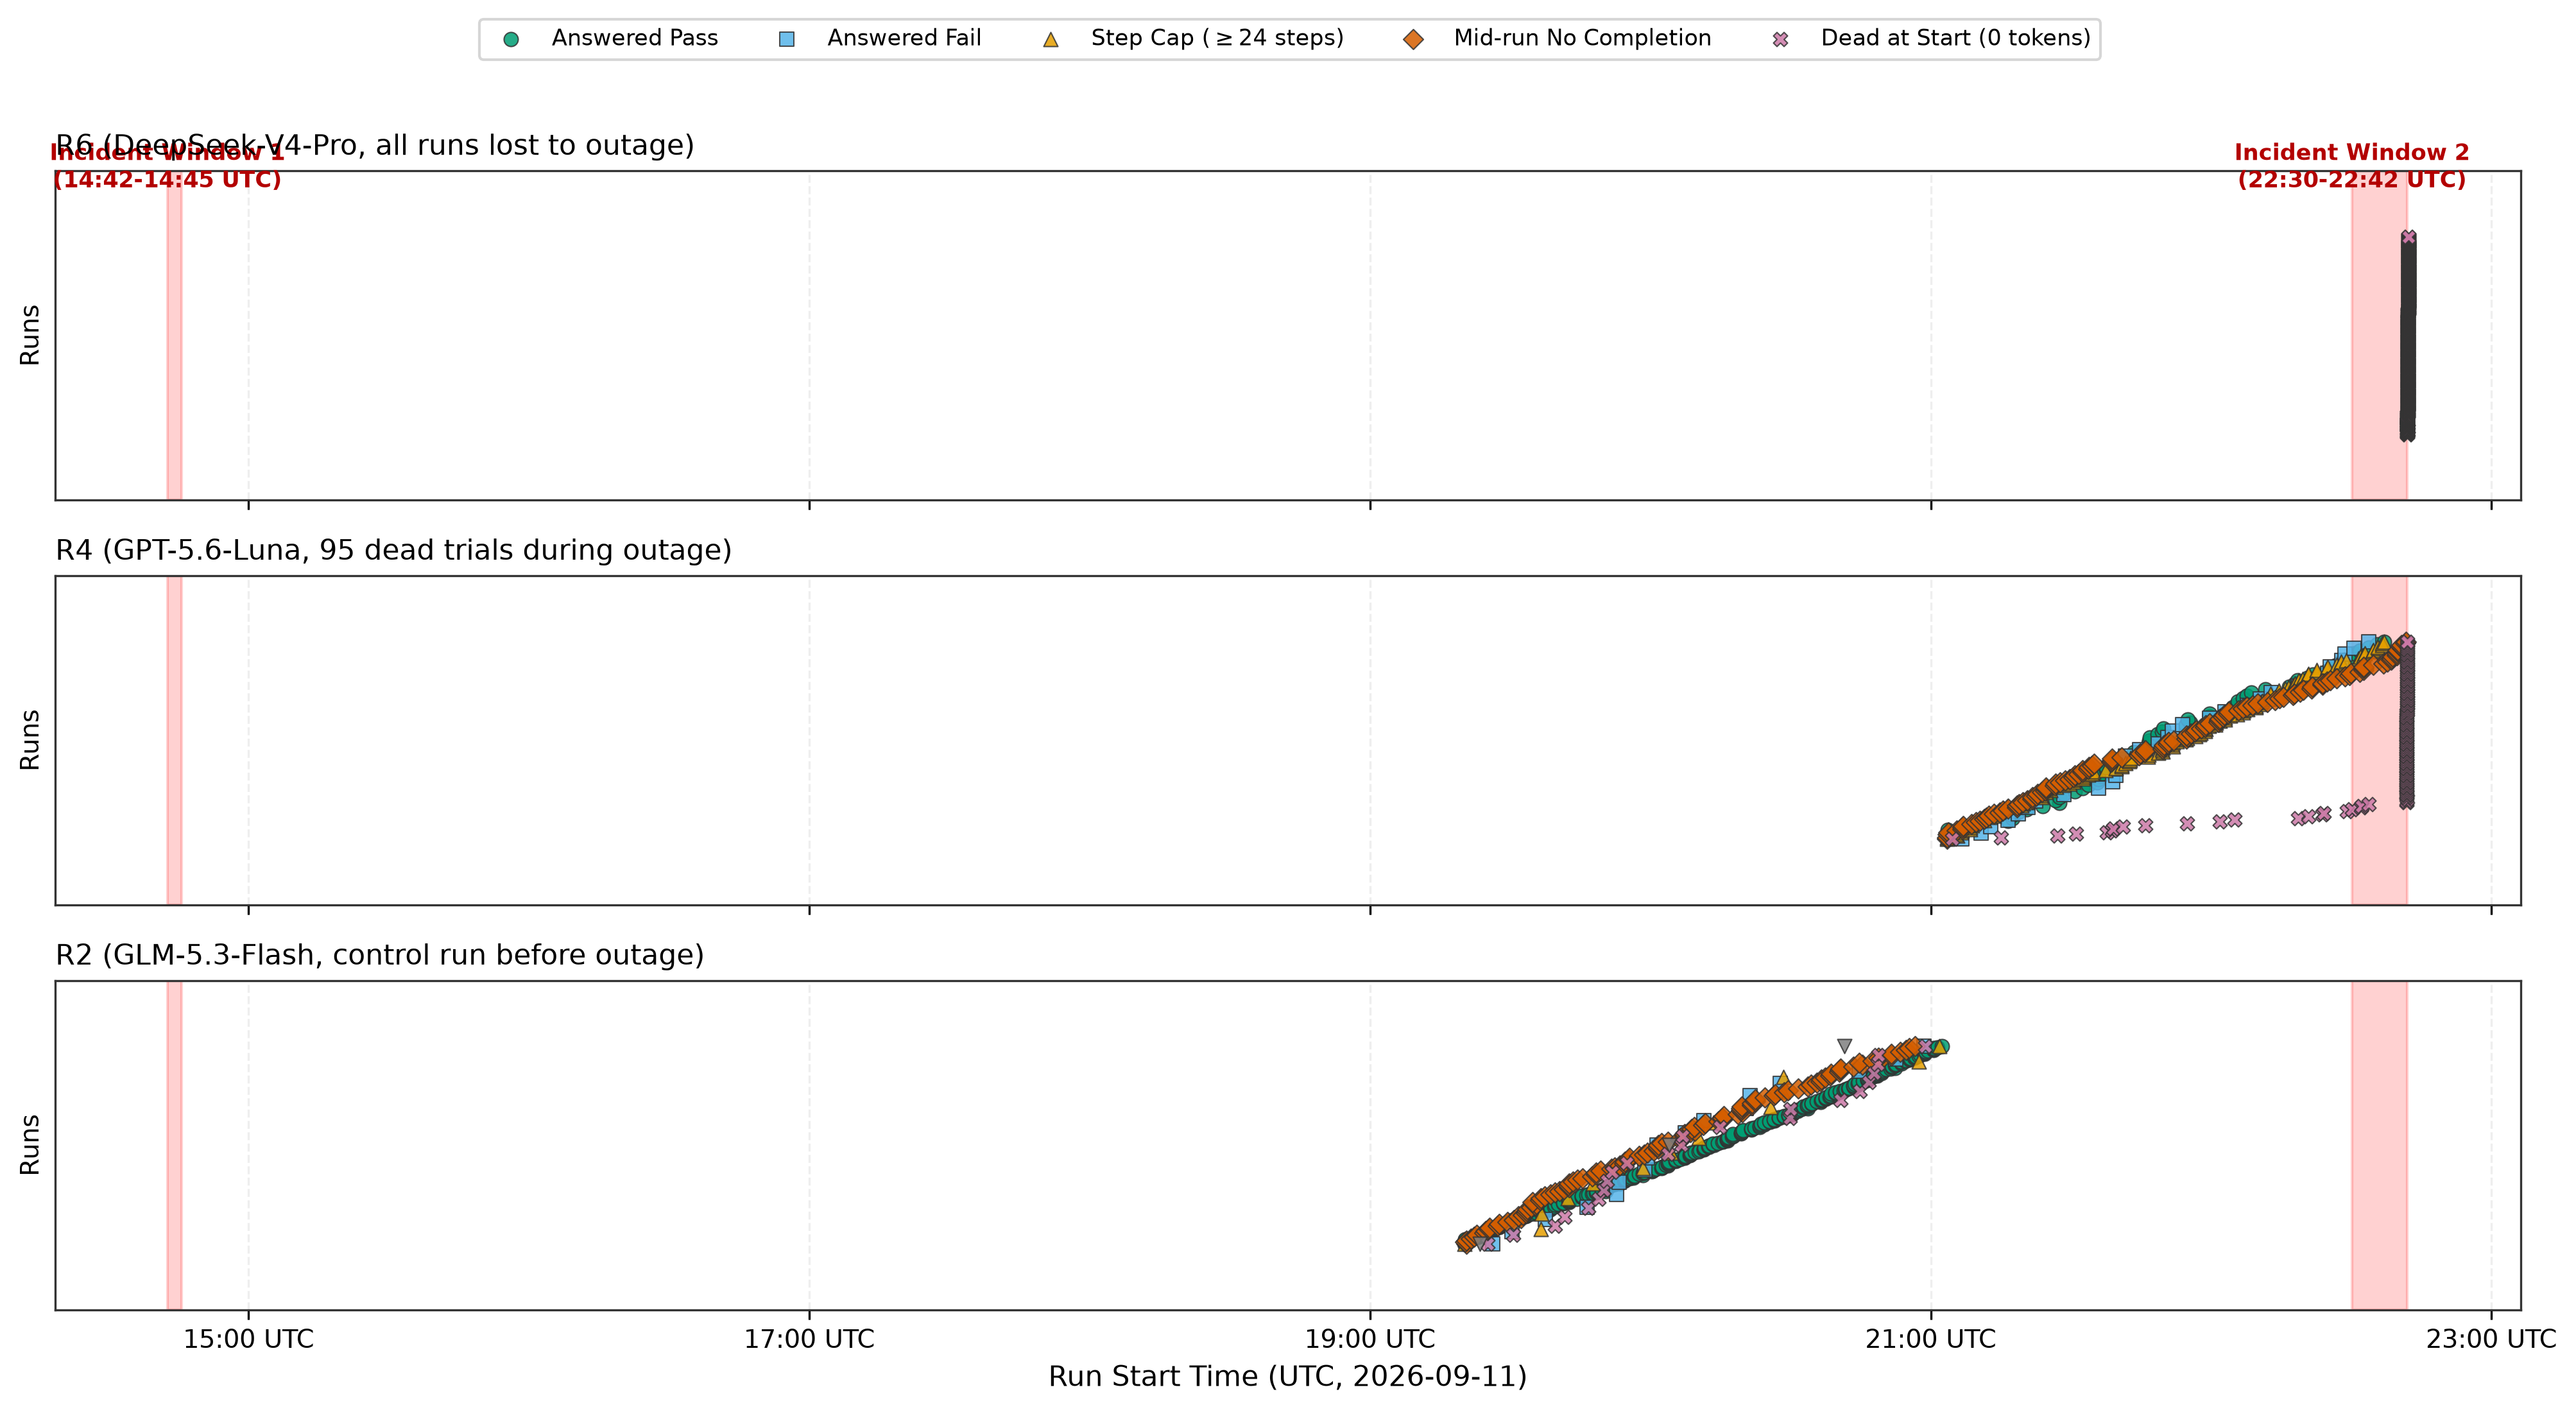
\includegraphics[width=0.95\textwidth]{fig_4_incident_timeline.png}
\caption{Figure 4: Per-trial execution timeline and terminal states across R6, R4, and R2 final pass runs on 2026-09-11 UTC. Shaded bands indicate the two gateway outage windows (14:42–14:45 UTC and 22:30–22:42 UTC). R6 suffered 100\% dead-at-start runs ($n=450$ trials) due to gateway step-1 connection drops. R4 experienced 95 dead trials (87 with $<1$ ms latency from client-side circuit breaker trips). R2 executed prior to the outage with 0 dead trials.}
\label{fig:fig_4_incident_timeline_png}
\end{figure}


We register a post-hoc sensitivity exclusion rule (Decision D-008):
- \textbf{Exclusion Rule:} A trial is \emph{infrastructure-dead} iff every span of that \texttt{(run\_id, scenario\_id)} has \texttt{completion\_tokens == 0} (or \texttt{None}) AND \texttt{max(step\_index) <= 1} [D-008]. A scenario is dropped if it experienced $\ge 1$ dead trial [D-008].

R2 had 0 dead trials ($n=150$). For R4, 33 scenarios are dropped, leaving $n=117$ valid scenarios (351 trials). We report the pre-registered \emph{as-run} analysis ($n=150$) as the primary evaluation and the \emph{infra-excluded} sensitivity analysis ($n=117$) alongside it to measure the impact of external dropouts [D-008]. Additionally, we evaluate a strict sensitivity variant (\emph{infra\_excluded\_strict}) that purges scenarios experiencing any midrun timeout or dead trial in Pass 2 (retaining $n=49$ for R2 and $n=24$ for R4).

\subsection{Attempt Segmentation and Final-Pass Isolation}
Forensic analysis of \texttt{projects/p06\_passk/trace.db} (Decision D-010) revealed that the database contains two chronological execution passes: Pass 1 under step cap 12 (12:15–14:47 UTC) and Pass 2 under step cap 24 (19:20–22:42 UTC). Because \texttt{record\_verdict} updated all spans for a run upon completion, the stored verdicts in \texttt{trace.db} correspond to Pass 2. First-pass verdicts are unrecoverable because raw completion text was not stored. Pass 1 consumed 18,917,495 tokens (\$0.3974 USD discarded spend), while Pass 2 consumed 35,401,507 tokens (\$23.0719 USD final spend), for a grand total of 54,319,002 tokens and \$23.4693 USD across 1,800 runs (34.83\% tokens discarded).

To avoid mixing step caps and invalidating span counts, all span-level metrics—including token usage, terminal-state classifications, and cost per grounded pass—are strictly computed on Pass 2 spans isolated via timestamp bounds [D-010]. Under Pass 2 isolation, zero runs terminate at step 12 (\texttt{step\_cap\_sub24 = 0}).

\section{Results}

We report findings in the strict order: \textbf{RAW RESULT}, \textbf{DERIVED RESULT}, and \textbf{INTERPRETATION}.

\subsection{Raw Results}
Raw counts from \texttt{analysis.json} and \texttt{p06\_results.md}:
- \textbf{R2 (\texttt{z-ai/glm-5.3-flash}, as-run, $n=150$, 450 trials):} 284 passes out of 450 trials. Observed histogram: $\{0: 8, 1: 34, 2: 74, 3: 34\}$. Concentration counts: 3-pass = 34, mixed = 108, 0-pass = 8. Dead trials: 0. Final-pass spend: \$5.0994 USD (\$5.1485 USD across passes; \$0.01796 per grounded pass). Pass 2 terminal states: answered\_pass = 284, midrun\_no\_completion = 109, step\_cap ($\ge$ 24) = 14, dead\_at\_start = 23, answered\_fail = 17, other = 3, step\_cap\_sub24 = 0. Latency signatures: midrun\_no\_completion exhibits 104 spans $>60$ s.
- \textbf{R4 (\texttt{openai/gpt-5.6-luna}, as-run, $n=150$, 450 trials):} 67 passes out of 450 trials. Observed histogram: $\{0: 95, 1: 46, 2: 6, 3: 3\}$. Concentration counts: 3-pass = 3, mixed = 52, 0-pass = 95. Dead trials: 95 across 33 scenarios (31 all-3 dead; split: $k_1=31, k_2=32, k_3=32$; window: 14:42:37 to 22:41:55 UTC). Final-pass spend: \$17.9725 USD (\$18.3208 USD across passes; \$0.26825 per grounded pass). Pass 2 terminal states: step\_cap ($\ge$ 24) = 118, midrun\_no\_completion = 119, answered\_pass = 67, dead\_at\_start = 114, answered\_fail = 32, other = 0, step\_cap\_sub24 = 0. Latency signatures: dead\_at\_start exhibits 106 spans $<1$ ms (breaker fast-fail), 2 spans $>60$ s (timeouts); midrun\_no\_completion exhibits 100 spans $>60$ s.
- \textbf{R4 (\texttt{openai/gpt-5.6-luna}, infra-excluded, $n=117$, 351 trials):} 67 passes out of 351 trials. Observed histogram: $\{0: 62, 1: 46, 2: 6, 3: 3\}$. Concentration counts: 3-pass = 3, mixed = 52, 0-pass = 62.
- \textbf{R6 (\texttt{deepseek/deepseek-v4-pro}, invalid):} 450 runs, 900 spans, 0 verdicts (869 spans $<1$ ms, 12 timeouts $>60$ s) [C023, C031]. Spend: \$0.07 USD.
- \textbf{Sweep Cumulative Spend \& Attempts Breakdown:} Pass 1 (cap 12) consumed 18,917,495 tokens (\$0.3974 USD discarded); Pass 2 (cap 24) consumed 35,401,507 tokens (\$23.0719 USD final spend); grand total across all 1,800 runs was 54,319,002 tokens and \$23.4693 USD (34.83\% tokens discarded from Pass 1) [C024, C067].

\subsection{Derived Results}

\subsubsection*{Primary Consistency, Goodness-of-Fit, and Overdispersion}
Table 1 presents consistency metrics, confidence intervals, concentration ratios, and goodness-of-fit statistics across model tiers. Table 2 details observed versus expected successes-per-scenario distributions.


\begin{table}[htbp]
\centering
\scriptsize
\setlength{\tabcolsep}{2.0pt}
\resizebox{\textwidth}{!}{
\begin{tabular}{lcccccccc}
\toprule
Model Tier \& Analysis & Scenarios ($n$) & Measured $\text{pass@1}$ [95\% CI] & Measured $\text{pass}^3$ [95\% CI] & Naive $(\text{pass@1})^3$ [Bootstrap CI] & Concentration Ratio $C_3$ [Bootstrap CI] & Goodness-of-Fit $\chi^2$ (df=2) [Param MC $p$] & Tarone $Z$ Score [$p$-value] & $\text{ICC}(1,1)$ [Bootstrap CI] \\
\midrule
\textbf{R2 (as-run)} & 150 & 0.6311 [0.5856, 0.6744] & 0.2267 [0.1670, 0.3000] & 0.2514 [0.2019, 0.3053] & 0.9017 [0.7161, 1.0793] & 1.8919 [$p=0.3794$] & $z=-0.655$ [$p=0.7438$] & -0.0287 [-0.1217, 0.0668] \\
\textbf{R4 (as-run)} & 150 & 0.1489 [0.1190, 0.1847] & 0.0200 [0.0068, 0.0571] & 0.0033 [0.0015, 0.0065] & 6.0596 [0.0000, 12.7450] & 13.6052 [$p=0.0053$] & $z=1.869$ [$p=0.0308$] & 0.0905 [-0.0499, 0.2347] \\
\textbf{R4 (infra-excluded)} & 117 & 0.1909 [0.1532, 0.2353] & 0.0256 [0.0088, 0.0727] & 0.0070 [0.0033, 0.0128] & 3.6867 [0.0000, 7.5772] & 7.8047 [$p=0.0243$] & $z=0.764$ [$p=0.2224$] & 0.0438 [-0.0978, 0.1907] \\
\bottomrule
\end{tabular}
}
\caption{Table 1: Multi-trial consistency metrics ($k=3$). Single-trial pass@1 proportions report 95\% Wilson score intervals assuming trial-level exchangeability ($n=450$ trials; scenario-level bootstrap CIs are $[0.5867, 0.6733]$ for R2, $[0.1133, 0.1867]$ for R4 as-run, and $[0.1481, 0.2336]$ for R4 infra-excluded); naive predictions, $C_3 = \text{pass}^3 / (\text{pass@1})^3$, and $\text{ICC}(1,1)$ report 95\% scenario-level percentile bootstrap intervals (10,000 resamples, $n=150$ scenarios). Goodness-of-fit reports Pearson $\chi^2$ test with parametric bootstrap $p$-values ($\text{df}=2$) against the homogeneous-binomial null $\text{Binomial}(3, \text{pass@1})$. Tarone $Z$ reports the $C(\alpha)$ test for binomial goodness-of-fit against beta-binomial overdispersion.}
\end{table}


\textbf{R2 Homogeneous Binomial Null:} As reported in Table 1, R2 achieves $\text{pass@1} = 0.6311$ (Wilson CI $[0.5856, 0.6744]$; bootstrap CI $[0.5867, 0.6733]$) and joint reliability $\text{pass}^3 = 0.2267$ (34/150; Wilson CI $[0.1670, 0.3000]$; bootstrap CI $[0.1600, 0.2933]$), closely matching naive compounding $(\text{pass@1})^3 = 0.2514$ (bootstrap CI $[0.2019, 0.3053]$). With $\Delta_3 = -0.0247$, concentration ratio $C_3 = 0.9017$ (bootstrap CI $[0.7161, 1.0793]$) comfortably spans 1.0. Pearson goodness-of-fit yields $\chi^2 = 1.8919$ ($\text{df}=2$, parametric bootstrap $p = 0.3794$, exact upper tail $p = 0.7840$), indicating that observed successes-per-scenario ($\{8, 34, 74, 34\}$ vs expected $\{7.53, 38.65, 66.12, 37.71\}$ in Table 2) are not distinguishable from the homogeneous-binomial null. Tarone's score test for overdispersion confirms the absence of clustering: $z = -0.655$ ($p = 0.7438, S = 140.735$). Intra-scenario correlation is null: $\text{ICC}(1,1) = -0.0287$ (bootstrap CI $[-0.1217, 0.0668]$) and Fleiss' $\kappa = -0.0309$ (bootstrap CI $[-0.1235, 0.0644]$).

\textbf{R4 Failure Concentration and Infrastructure Attenuation:} For R4 as-run ($n=150$), $\text{pass@1} = 0.1489$ (Wilson CI $[0.1190, 0.1847]$; bootstrap CI $[0.1133, 0.1867]$). Measured $\text{pass}^3$ is 0.0200 (3/150; Wilson CI $[0.0068, 0.0571]$; bootstrap CI $[0.0000, 0.0467]$) vs naive 0.0033 (bootstrap CI $[0.0015, 0.0065]$), yielding point $C_3 = 6.0596$ and $\Delta_3 = +0.0167$. While as-run data exhibits marginal overdispersion (Tarone $z = 1.869, p = 0.0308, S = 176.433$; parametric bootstrap GoF $p = 0.0053$), this effect is heavily driven by 95 infrastructure dropouts clustering in the 0-pass cell. Under infra-excluded sensitivity analysis ($n=117$), purging 33 dropout scenarios raises $\text{pass@1}$ to 0.1909 (Wilson CI $[0.1532, 0.2353]$; bootstrap CI $[0.1481, 0.2336]$). Measured $\text{pass}^3 = 0.0256$ (3/117; Wilson CI $[0.0088, 0.0727]$; bootstrap CI $[0.0000, 0.0598]$) vs naive 0.0070 (bootstrap CI $[0.0033, 0.0128]$), giving $\Delta_3 = +0.0187$ and point $C_3 = 3.6867$. Overdispersion evaporates once dropouts are removed: Tarone $z = 0.764$ ($p = 0.2224, S = 126.543$) and exact binomial tail $p = 0.0488$ on 3 vs 0.81 expected. The bootstrap CI on $C_3$ spans $[0.0000, 7.5772]$ (where the zero lower bound is a small-count artifact of 3 observed 3-pass scenarios appearing in zero draws for $\approx 4.8\%$ of resamples), encompassing 1.0, while $\text{ICC}(1,1)$ attenuates to 0.0438 (bootstrap CI $[-0.0978, 0.1907]$) and Fleiss' $\kappa$ to 0.0408 (bootstrap CI $[-0.1004, 0.1875]$).

\textbf{Strict Sensitivity Variant:} To ensure results are not confounded by soft-timeout runs, the strict sensitivity variant (\emph{infra\_excluded\_strict}) purges any scenario experiencing a midrun timeout ($>60$ s) or dead trial in Pass 2. R2 retains $n=49$ scenarios ($\text{pass@1} = 0.8776$, $\text{pass}^3 = 0.6939$ vs naive $0.6758$, $C_3 = 1.0267$ [CI $0.8654, 1.1578$], parametric bootstrap GoF $p = 0.4475$), remaining consistent with independence within confidence intervals. R4 retains $n=24$ scenarios ($\text{pass@1} = 0.3889$, $\text{pass}^3 = 0.1250$ vs naive $0.0588$, $C_3 = 2.1262$ [CI $0.0000, 4.4172$], parametric bootstrap GoF $p = 0.2787$), where the apparent departure from independence attenuates entirely.


\begin{table}[htbp]
\centering
\footnotesize
\setlength{\tabcolsep}{3.0pt}
\resizebox{\textwidth}{!}{
\begin{tabular}{lcccccc}
\toprule
Model Tier \& Analysis & $c_i = 0$ Pass (Obs / Exp) & $c_i = 1$ Pass (Obs / Exp) & $c_i = 2$ Pass (Obs / Exp) & $c_i = 3$ Pass (Obs / Exp) & Exact Tail $p$ ($c_i = 3$) & Parametric MC $p$ \\
\midrule
\textbf{R2 (as-run, $n=150$)} & 8 / 7.53 & 34 / 38.65 & 74 / 66.12 & 34 / 37.71 & 0.7840 & 0.3794 \\
\textbf{R4 (as-run, $n=150$)} & 95 / 92.48 & 46 / 48.53 & 6 / 8.49 & 3 / 0.50 & 0.0138 & 0.0053 \\
\textbf{R4 (infra-excluded, $n=117$)} & 62 / 61.98 & 46 / 43.86 & 6 / 10.35 & 3 / 0.81 & 0.0488 & 0.0243 \\
\bottomrule
\end{tabular}
}
\caption{Table 2: Observed vs expected successes-per-scenario distributions ($c_i \in \{0, 1, 2, 3\}$). Expected counts derived under $c_i \sim \text{Binomial}(3, \text{pass@1})$.}
\end{table}


Figure 1 plots the observed successes-per-scenario distributions alongside the theoretical Binomial(3, pass@1) null. Figure 2 compares measured multi-trial pass rates against naive compounding predictions across $k \in \{1, 2, 3\}$.


\begin{figure}[htbp]
\centering
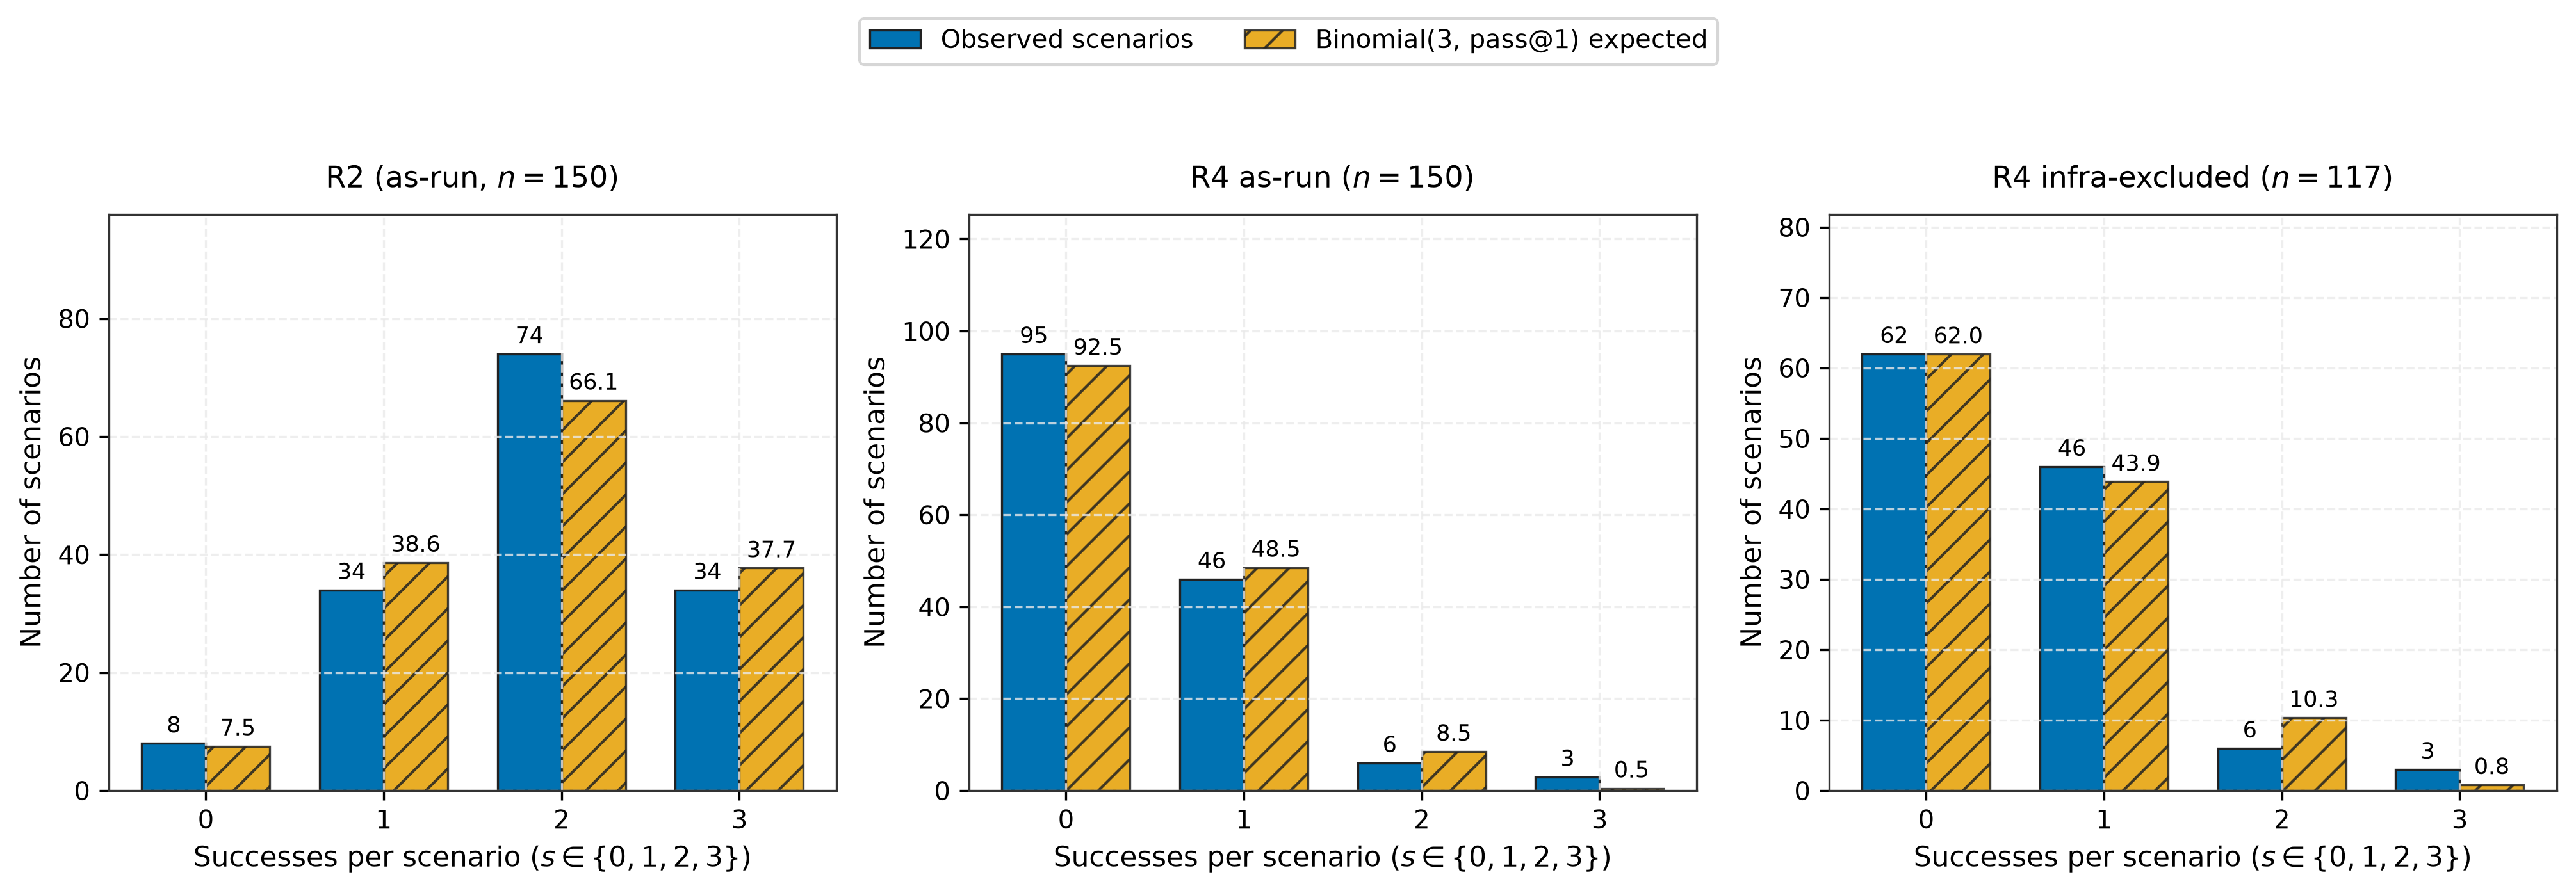
\includegraphics[width=0.95\textwidth]{fig_1_successes_per_scenario.png}
\caption{Figure 1: Observed versus Binomial(3, pass@1) expected scenario counts across success counts $s \in \{0, 1, 2, 3\}$. Panel A: R2 ($n=150$, $\chi^2 = 1.8919, p = 0.3794$). Panel B: R4 as-run ($n=150$, $\chi^2 = 13.6052, p = 0.0053$). Panel C: R4 infra-excluded ($n=117$, $\chi^2 = 7.8047, p = 0.0243$). Expected counts follow the homogeneous binomial model with $\hat{p} = \text{pass@1}$.}
\label{fig:fig_1_successes_per_scenario_png}
\end{figure}



\begin{figure}[htbp]
\centering
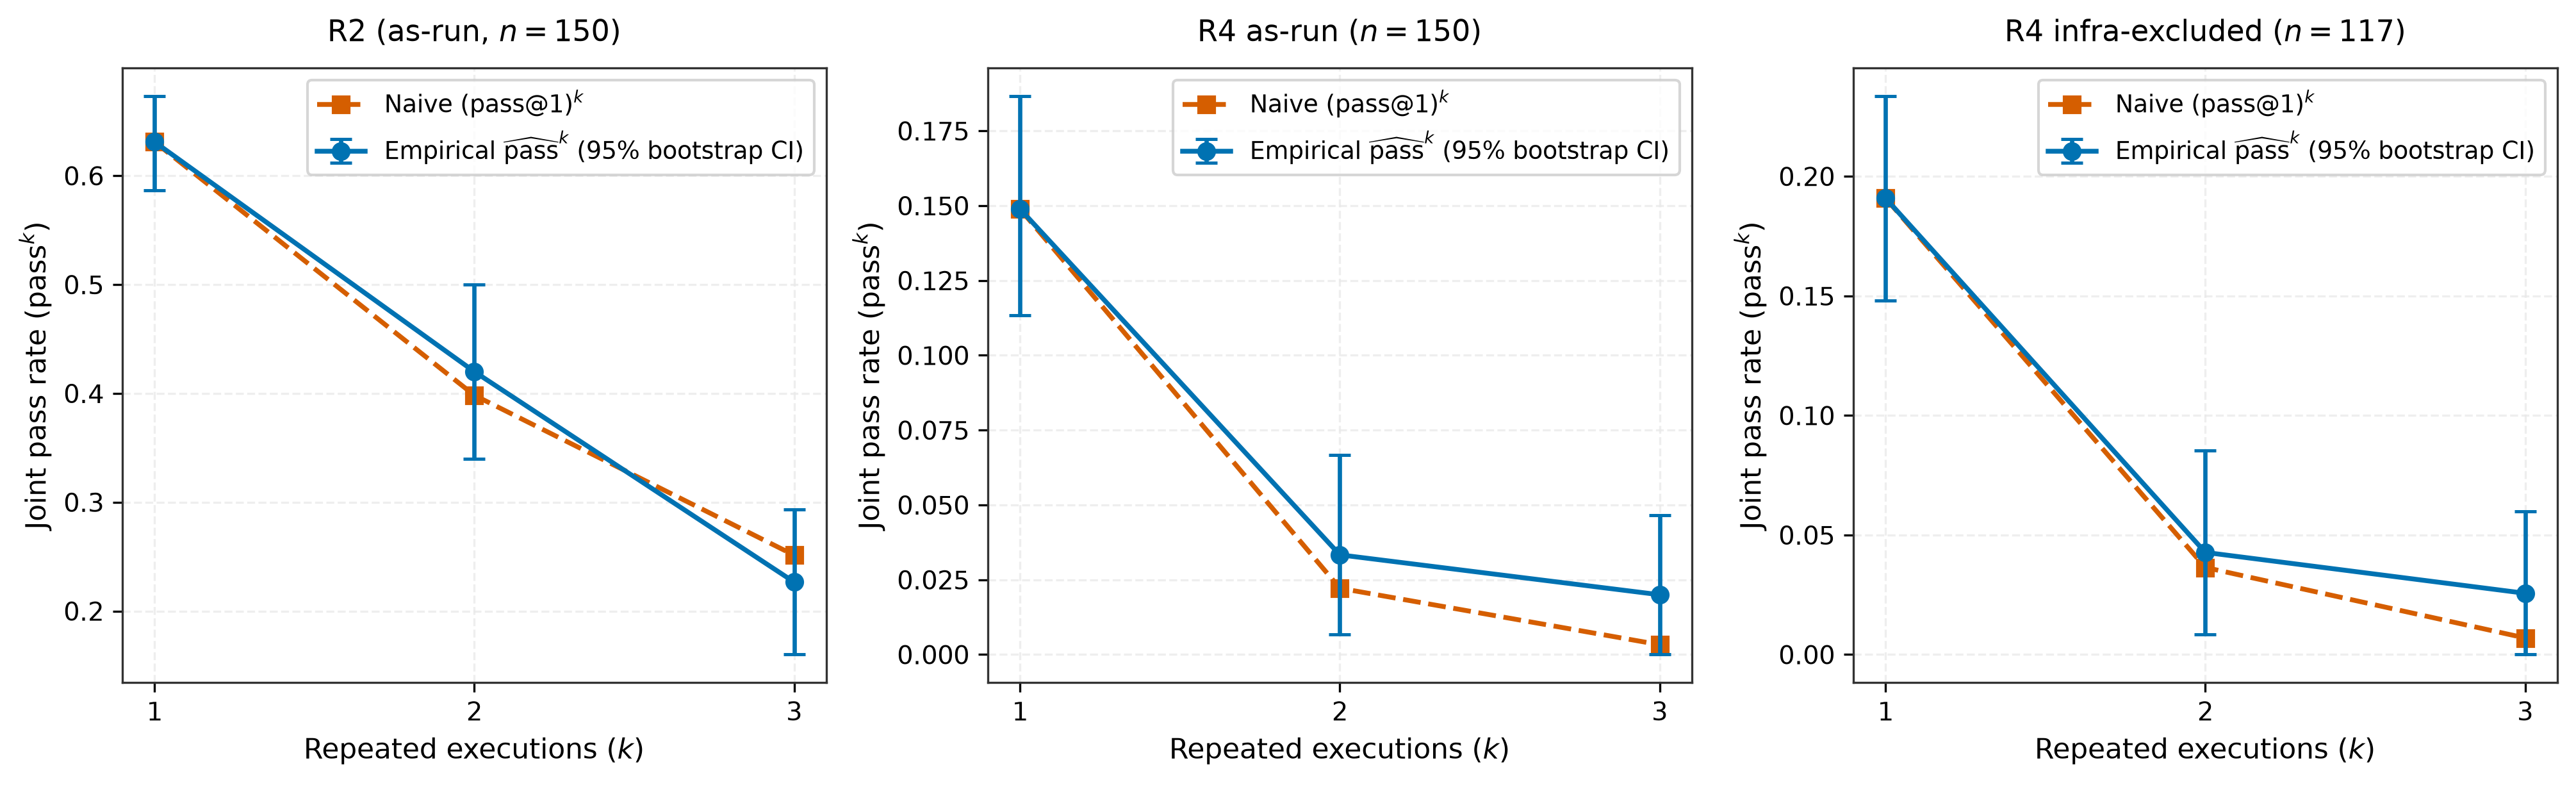
\includegraphics[width=0.95\textwidth]{fig_2_passk_vs_naive.png}
\caption{Figure 2: Empirical joint reliability $\widehat{\text{pass}}^k$ with 95\% scenario-level bootstrap confidence intervals compared against naive compounding $(\text{pass@1})^k$ for $k \in \{1, 2, 3\}$. Panel A: R2 ($n=150$, $\text{pass}^3 = 0.2267$ vs naive $0.2514$). Panel B: R4 as-run ($n=150$, $\text{pass}^3 = 0.0200$ vs naive $0.0033$). Panel C: R4 infra-excluded ($n=117$, $\text{pass}^3 = 0.0256$ vs naive $0.0070$).}
\label{fig:fig_2_passk_vs_naive_png}
\end{figure}


\subsubsection*{Paired Scenario Comparisons (R2 vs R4)}
Table 3 presents paired analyses on matched scenario IDs.


\begin{table}[htbp]
\centering
\footnotesize
\setlength{\tabcolsep}{3.0pt}
\resizebox{\textwidth}{!}{
\begin{tabular}{lcccccc}
\toprule
Comparison \& Sample & Discordant Pairs ($b$ R2-only / $c$ R4-only) & Risk Difference [Bootstrap CI] & Matched Odds Ratio [95\% CI] & Exact McNemar $p$ & Holm-Adjusted $p$ & Paired Cohen's $d_z$ \\
\midrule
\textbf{All-3-Pass (as-run, $n=150$)} & 34 / 3 & +0.2067 [0.1333, 0.2800] & 11.3333 [3.4808, 36.9004] & $1.23 \times 10^{-7}$ & $4.93 \times 10^{-7}$ & 0.46 \\
\textbf{Trial-1 Pass (as-run, $n=150$)} & 77 / 10 & +0.4467 [0.3467, 0.5400] & 7.7000 [3.9844, 14.8804] & $5.92 \times 10^{-14}$ & $2.96 \times 10^{-13}$ & 0.72 \\
\textbf{All-3-Pass (infra-excluded, $n=117$)} & 22 / 3 & +0.1624 [0.0855, 0.2393] & 7.3333 [2.1949, 24.5013] & $1.57 \times 10^{-4}$ & $4.70 \times 10^{-4}$ & 0.37 \\
\textbf{Trial-1 Pass (infra-excluded, $n=117$)} & 55 / 10 & +0.3846 [0.2650, 0.5043] & 5.5000 [2.8037, 10.7892] & $1.18 \times 10^{-8}$ & $4.70 \times 10^{-8}$ & 0.60 \\
\bottomrule
\end{tabular}
}
\caption{Table 3: Paired comparisons on identical scenario IDs. For All-3-Pass (as-run), ties $= 113$ (0 concordant pass, 113 concordant fail). For Trial-1 Pass (as-run), ties $= 63$ (13 concordant pass, 50 concordant fail). Holm-adjusted $p$-values computed across the primary family of 5 tests.}
\end{table}


In matched paired comparisons, R2 outperforms R4 across both metrics (All-3-Pass risk difference $+0.2067$, exact McNemar $p = 1.23 \times 10^{-7}$; Trial-1 Pass risk difference $+0.4467$, exact McNemar $p = 5.92 \times 10^{-14}$). Under the strict sensitivity variant ($n=14$ paired scenarios surviving), R2 maintains higher accuracy (Trial-1 exact McNemar $p = 0.0312$, 5 R2-only vs 0 R4-only; All-3-Pass exact McNemar $p = 0.1250$, 3 R2-only vs 0 R4-only).

\subsubsection*{Compounding Extrapolation across Depth $k=1..10$}
To evaluate the practical consequences of small intra-scenario correlations at higher depths, Table 4 presents beta-binomial compounding extrapolations across $k \in \{1, \dots, 10\}$ for R2.


\begin{table}[htbp]
\centering
\small
\setlength{\tabcolsep}{4.5pt}
\resizebox{\textwidth}{!}{
\begin{tabular}{lcccc}
\toprule
Depth $k$ & Naive Prediction $(\text{pass@1})^k$ & Beta-Binomial Expected $\text{pass}^k$ & Concentration Ratio $C_k$ (Point Estimate) & Concentration Ratio $C_k$ (at $\text{ICC}_{\text{hi}} = 0.0668$) \\
\midrule
$k=1$ & 0.6311 & 0.6311 & 1.00 & 1.00 \\
$k=2$ & 0.3983 & 0.3983 & 1.00 & 1.04 \\
$k=3$ & 0.2514 & 0.2514 & 1.00 & 1.10 \\
$k=4$ & 0.1586 & 0.1586 & 1.00 & 1.21 \\
$k=5$ & 0.1001 & 0.1001 & 1.00 & 1.39 \\
$k=6$ & 0.0632 & 0.0632 & 1.00 & 1.60 \\
$k=7$ & 0.0399 & 0.0399 & 1.00 & 1.89 \\
$k=8$ & 0.0252 & 0.0252 & 1.00 & 2.25 \\
$k=9$ & 0.0159 & 0.0159 & 1.00 & 2.74 \\
$k=10$ & 0.0100 & 0.0100 & 1.00 & 3.36 \\
\bottomrule
\end{tabular}
}
\caption{Table 4: Beta-binomial compounding extrapolation across repetition depths $k \in \{1, \dots, 10\}$ for R2 ($\text{pass@1} = 0.6311$). While $C_3 \approx 1.10$ at $k=3$ (a 1.4 pp gap), divergence amplifies to $C_8 \approx 2.25$ by $k=8$ ($\text{pass}^8 \approx 0.057$ vs naive $0.025$).}
\end{table}


Figure 3 displays the compounding extrapolation across depths $k=1..10$ for R2 and R4 (both variants), demonstrating why consistency at $k=3$ cannot license compounding claims at higher depths.


\begin{figure}[htbp]
\centering
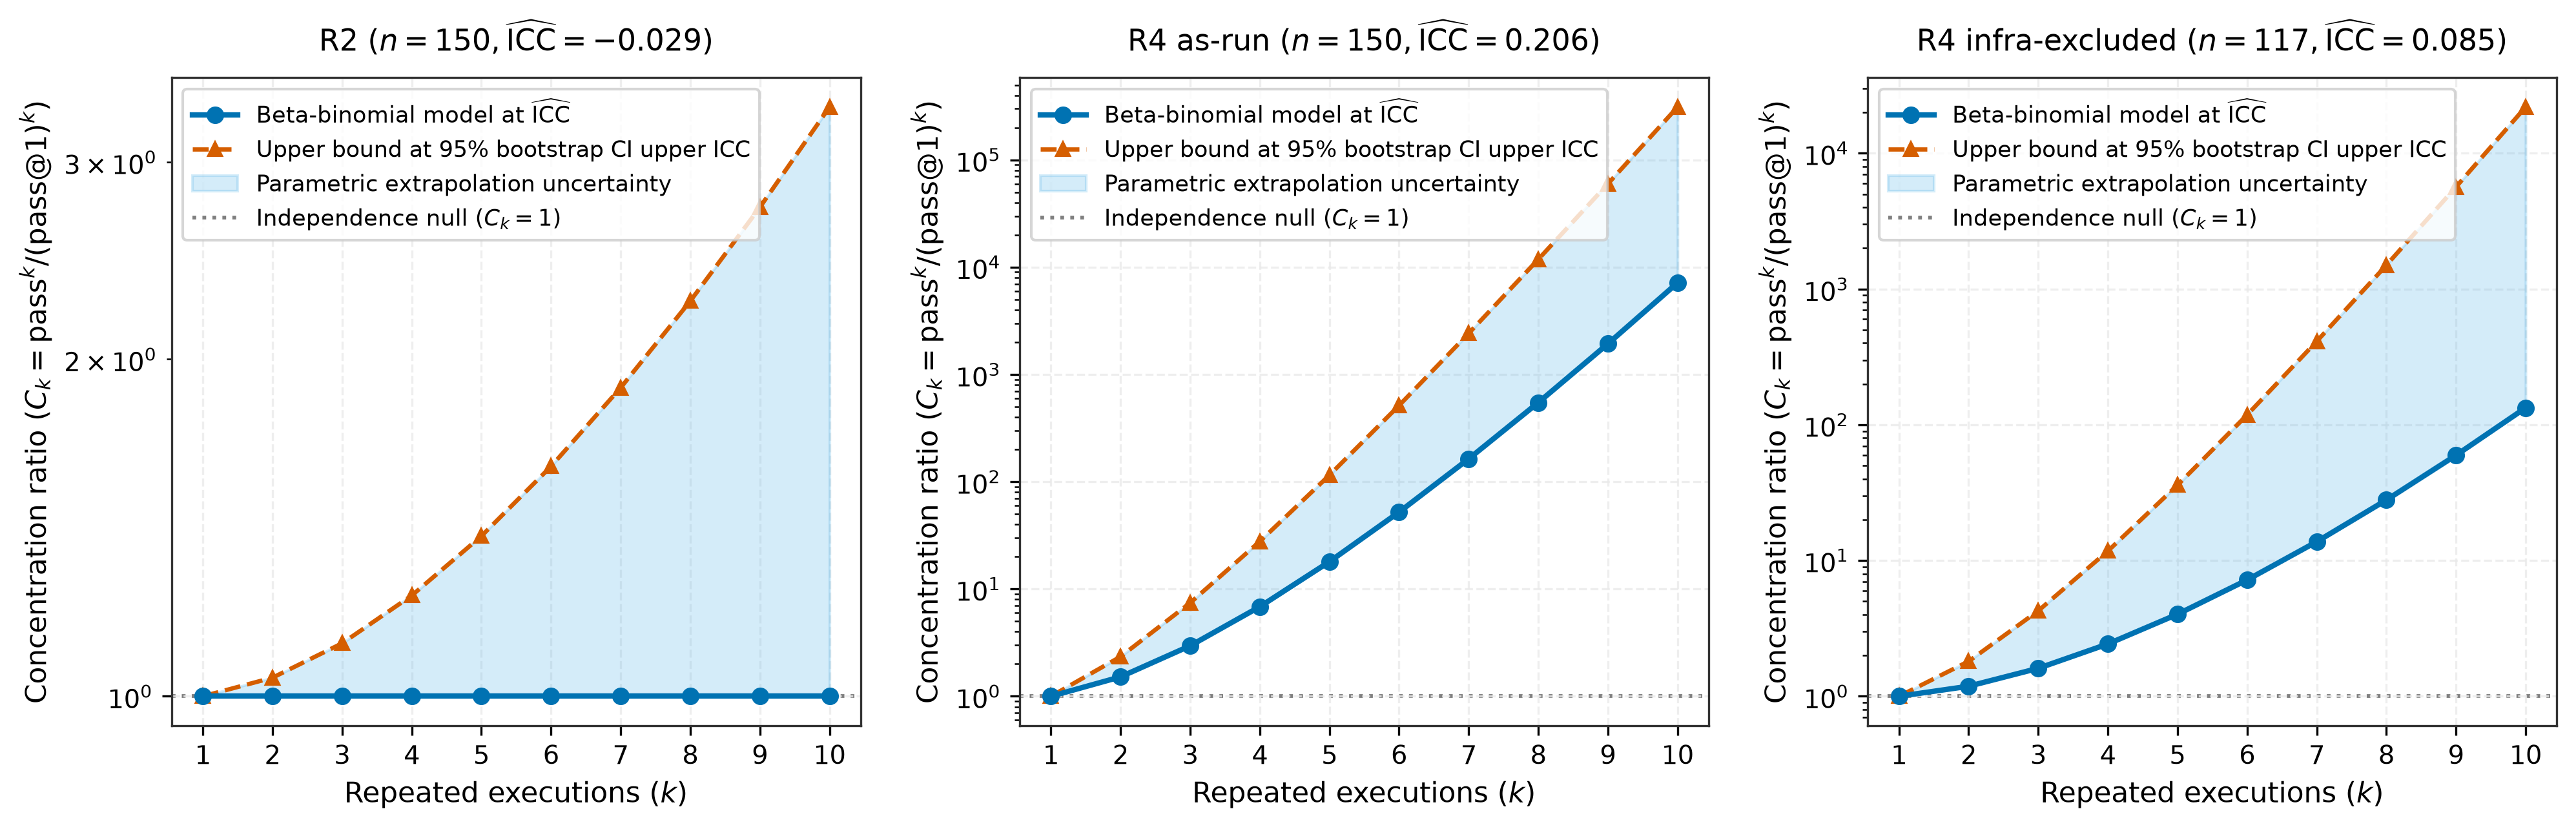
\includegraphics[width=0.95\textwidth]{fig_3_icc_extrapolation.png}
\caption{Figure 3: Implied concentration ratio $C_k = \text{pass}^k / (\text{pass@1})^k$ extrapolated across depth $k=1..10$ under the beta-binomial model. Panel A: R2 ($n=150, \widehat{\text{ICC}} = -0.0287$, capped at 0). Panel B: R4 as-run ($n=150, \widehat{\text{ICC}} = 0.2057$, upper 95\% bootstrap bound $\text{ICC} = 0.3804$). Panel C: R4 infra-excluded ($n=117$, $\widehat{\text{ICC}} = 0.0849$, upper 95\% bootstrap bound $\text{ICC} = 0.2642$). The dotted line marks the independence null $C_k = 1.0$.}
\label{fig:fig_3_icc_extrapolation_png}
\end{figure}


\subsubsection*{Hypothesis Verdicts}
Both pre-registered hypotheses are unresolved under pre-registered rules due to design shortfall:
- \textbf{Hypothesis H4:} NOT\_TESTABLE\_AS\_PREREGISTERED (2 of 6 rungs valid). The pre-registered rule required $\ge 4$ of 6 rungs to evaluate. On the 2 valid rungs, the pre-registered per-rung criterion (Wilson CI of measured $\text{pass}^3$ excludes and exceeds naive $(\text{pass@1})^3$) held on R4 under both as-run (Wilson CI $[0.0068, 0.0571]$ vs naive $0.0033$) and infra-excluded (Wilson CI $[0.0088, 0.0727]$ vs naive $0.0070$) analyses, but did not hold on R2 (Wilson CI $[0.1670, 0.3000]$ contained naive $0.2514$). Note that this per-rung criterion treats the naive prediction as fixed; parametric bootstrap goodness-of-fit and exact tail tests properly account for sampling error in $\text{pass@1}$.
- \textbf{Hypothesis H5:} NOT\_TESTABLE\_AS\_PREREGISTERED (2 of 6 rungs valid). Testing monotonic ordering requires a multi-tier ladder across $\ge 4$ rungs; with 2 valid rungs, rank correlation is degenerate. Point estimates show $\Delta_{R2} = -0.0247$ vs $\Delta_{R4} = +0.0167$ (as-run) and $\Delta_{R4} = +0.0187$ (infra-excluded), reversing the hypothesized ordering, but the difference $\Delta_{R4} - \Delta_{R2} = +0.0414$ has a 95\% scenario bootstrap CI of $[-0.0080, 0.0922]$ which includes zero and is not statistically distinguishable from null.

\subsection{Interpretation}
[we interpret] Drawing together the evidence, we interpret these results under four core findings:
1. \textbf{Remarkable Accuracy of Naive Compounding at $k=3$:} Across both evaluated model tiers, naive independent Bernoulli compounding is within 2.5 percentage points of measured joint reliability ($\Delta_3 = -0.0247$ on R2; $\Delta_3 = +0.0187$ on R4 infra-excluded). In both cases, the deviation and its upper 95\% bootstrap confidence bound ($+0.048$) are far below our pre-registered 10 percentage point minimum effect of interest.
2. \textbf{Homogeneous Binomial Null Holds on R2:} On the evaluated higher-accuracy tier (R2), agent outcomes are not distinguishable from independent Bernoulli trials (parametric bootstrap GoF $p = 0.3794$, Tarone overdispersion $z = -0.655, p = 0.7438$, $\text{ICC} = -0.0287$). There is no detectable across-scenario task difficulty clustering or within-scenario serial dependence.
3. \textbf{Apparent Low-Accuracy Excess is Attenuated by Infrastructure Outages:} On R4, the apparent overdispersion is heavily driven by 95 network timeouts clustering in the 0-pass cell. Purging infrastructure dropouts evaporates overdispersion (Tarone $z = 0.764, p = 0.2224$), leaving a marginal 1.86 pp excess ($p = 0.0488$) and an unresolved concentration ratio ($C_3$ bootstrap CI $[0.0000, 7.5772]$ includes 1.0). Under strict exclusion of midrun timeouts ($n=24$), the departure attenuates entirely ($p = 0.2787$).
4. \textbf{Indistinguishability at $k=3$ versus Compounding Divergence at Scale:} At repetition depth $k=3$, observations cannot mathematically separate across-scenario task heterogeneity from within-scenario serial correlation. However, beta-binomial compounding extrapolation demonstrates that even undetectable intra-scenario correlation ($\text{ICC}_{\text{hi}} = 0.0668$) compounds into a $2.25\times$ divergence at $k=8$ ($\text{pass}^8 \approx 0.057$ vs naive $0.025$). Small departures at shallow evaluation depths compound into notable operational divergence at higher depths ($C_8 \approx 2.25$).



\section{Supporting Evidence: Diagnostic Sweep Failure Taxonomy}
\begin{quote}
\textbf{Provenance Caveat:} Experiments P3, P4, and P5 were preliminary diagnostic sweeps under MEC v1.2 with step cap 12 (Amendment A-002), prior to Amendment A-003 expanding the cap to 24 for primary experiment P6. P3 was contaminated by gateway rate limits. P4 human axial coding was performed on 200 traces from P3 by a single author. P5 judge calibration evaluated \texttt{z-ai/glm-5.3} on a frozen 60-trace test split of P4, belonging to the same model family as rung R2. None of P3, P4, or P5 data originates from the P6 runs upon which our main result rests. Findings here are designated as \textbf{SUPPORTING} (appendix-bound).
\end{quote}

In P3 diagnostic sweeps across 200 scenarios, accuracy collapsed as retrieval depth expanded: Tier 1 (1-hop) reached $\text{pass@1} = 1.0000$ (67/67; Wilson CI $[0.9458, 1.0000]$) requiring 4.01 steps and 2,633 tokens; Tier 2 (2–3 hops) reached $\text{pass@1} = 0.6119$ (41/67; Wilson CI $[0.4922, 0.7195]$) with 10.57 steps and 18,647 tokens; Tier 3 (5 hops) collapsed to $\text{pass@1} = 0.0758$ (5/66; Wilson CI $[0.0328, 0.1654]$) with 11.74 steps and 25,945 tokens. Disjoint Wilson intervals confirm diagnostic hypothesis H1: multi-hop depth degrades real-model pass rates.

Axial coding of 200 execution traces from P3 (17 passed, 183 failed; pass rate 0.085) revealed that failures stem from diverse structural pathologies. Beyond gateway rate limits (\texttt{INFRASTRUCTURE\_RATE\_LIMIT}, 114 traces, 62.30\%) and syntax errors (\texttt{MALFORMED\_TOOL\_CALL}, 23 traces, 12.57\%), the analysis uncovered five emergent failure modes absent from initial catalogs (confirming hypothesis H2): \texttt{OVERCONSTRAINED\_SEARCH\_LOOP} (36 traces, 19.67\%), \texttt{MULTI\_HOP\_TRAVERSAL\_EXHAUSTION} (3 traces, 1.64\%), \texttt{INFRASTRUCTURE\_SERVER\_ERROR} (3 traces, 1.64\%), \texttt{RETRIEVAL\_FAILURE\_ABSTENTION} (1 trace, 0.55\%), \texttt{ANSWER\_EXTRACTION\_TRUNCATION} (1 trace, 0.55\%), \texttt{PREMATURE\_STOP\_WRONG\_HOP} (1 trace, 0.55\%), and \texttt{MULTI\_HOP\_DIRECTION\_ERROR} (1 trace, 0.55\%). Full definitions appear in Appendix C.

In P5, automated evaluators were calibrated against human labels on a frozen $n=60$ test split. Hypothesis H3 was \textbf{FALSIFIED}: only 2 of 5 core modes met $\kappa \ge 0.70$. P5 also exposed mathematical fragility under class imbalance [17]. For four failure modes (\texttt{MULTI\_HOP\_TRAVERSAL\_EXHAUSTION}, \texttt{RETRIEVAL\_FAILURE\_ABSTENTION}, \texttt{ANSWER\_EXTRACTION\_TRUNCATION}, \texttt{MULTI\_HOP\_DIRECTION\_ERROR}), the test split contained zero human positives ($\text{tp} + \text{fn} = 0$). In these degenerate splits, evaluators predicting all-negative achieved 100\% TNR and $\kappa = 1.0$ (or 0.0), creating the illusion of perfect performance without positive detection capability [we interpret]. Full calibration data appears in Appendix D.



\section{Implications for Evaluation Practice}

1. \textbf{Do Not Assume Naive $(\text{pass@1})^k$ Compounding Holds:} [we interpret] System designers cannot assume naive independent Bernoulli compounding holds across all regimes; empirical multi-trial consistency should be measured directly rather than extrapolated from single-trial pass rates.
2. \textbf{Disclose Inference Backends and Report Instance-Level Error Bars:} Publishing point estimates obscures noise [15]. As shown by our bootstrap intervals, concentration ratios near zero are highly volatile ($C_3 \in [0.0000, 7.5772]$). Evaluators should report Wilson score intervals for proportions [22] and cluster-level bootstrap intervals for derived ratios [6]. Because temperature 0 does not ensure determinism [10, 16], papers must document serving engines, batch concurrency, and gateway configurations.
3. \textbf{Audit Traces for Client-Side Fast-Fails:} Client-side circuit breakers can silently convert transient remote timeouts into batches of $<1$ ms step-1 failures, inflating zero-pass counts. Benchmarking pipelines must record full exception text and conduct sensitivity analyses separating infrastructure dropouts from reasoning failures [D-008].
4. \textbf{Deploy Deterministic Dual-Condition Oracles:} Automated LLM judges suffer from position bias, verbosity bias, and reliability attenuation under class imbalance [17, 25]. Wherever feasible, agent benchmarks should grade completion using deterministic oracles that verify both normalized semantic outputs and explicit citation of ground-truth provenance.



\section{Related Work}

\subsection{Functional Code Generation and Multi-Trial Agent Reliability}
Chen et al. [2] formalized the unbiased $\text{pass@k}$ estimator for functional code generation, evaluating the probability that at least one of $k$ generated sample programs passes unit tests [C001, E001]. Yao et al. [23] introduced $\tau$-bench, formalizing joint reliability $\text{pass}^k$ for multi-turn tool interaction where an agent must successfully complete all $k$ repeated interaction episodes on a task instance, observing that high single-trial performance ($\text{pass@1}$) can mask severe multi-trial reliability degradation [C002, E002]. However, $\tau$-bench did not benchmark the empirical gap to $(\text{pass@1})^k$ or evaluate across-scenario heterogeneity versus within-scenario serial correlation; our work directly tests this compounding gap under repetition. Jiang et al. [12] demonstrated that multi-turn agent evaluations frequently conflate internal unit test assertions with independent agent rollouts, inflating reported operational reliability [C069, E009]. Bellibatlu et al. [1] showed that clinical decision agents can achieve nominal task success while executing discordant intermediate tool actions across repeated runs [C070, E010].

\subsection{Inference Nondeterminism at Temperature 0}
Greedy decoding at temperature 0 is widely assumed by practitioners to produce deterministic output across repeated API queries [C003, E003, E019, E020]. However, He et al. [10] demonstrated that modern GPU batching and parallel floating-point reductions cause non-zero output divergence even at temperature 0 [C004, E004]. Pape et al. [16] found that differing serving engines (vLLM, SGLang, llama.cpp) produce measurable output disagreement on fixed benchmarks at temperature 0, shifting benchmark scores by up to 16.6 percentage points [C071, E005]. Reddy et al. [18] showed that routing identical open-weight models across commercial API providers yields discordant task completions [C072, E006]. Fu et al. [8] also demonstrated that non-associative floating-point addition in GPU attention kernels alters token logits, occasionally flipping greedy argmax selection when candidate token probabilities are close [C073, E007].

\subsection{Statistical Foundations of Model Evaluation}
Miller [15] argues that language model evaluations are scientific experiments that should report standard errors and paired tests, noting that standard benchmark practice rarely tests claimed improvements for statistical significance [C005, E008]. Zheng et al. [25] documented systematic position, verbosity, and self-enhancement biases in automated model judges [C006, E011]. Rao and Callison-Burch [17] showed that percent agreement and kappa can diverge sharply depending on protocol choices and label prevalence under class imbalance [C012, E012]. Our evaluation methodology is grounded in classical statistical foundations: asymmetric Wilson score intervals [22] [C007, E013], paired exact McNemar tests conditioned on discordant observation pairs [14] [C008, E014], Rogan-Gladen prevalence estimation [19] [C074, E015], one-way random effects intraclass correlation [20] [C075, E016], percentile bootstrap resampling [6] [C076, E017], and sequentially rejective Holm-Bonferroni testing [11] [C077, E018].

\section{Limitations}

[limitation] We explicitly document nine threats to validity and scope constraints:
1. \textbf{Single Synthetic Environment:} Evaluations were conducted exclusively on a synthetic 300-entity pseudoword knowledge graph. While synthetic graphs eliminate pre-training contamination, they do not replicate the syntactic variety of unstructured web documents or noisy production databases.
2. \textbf{Two Valid Model Tiers:} Following the invalidation of R6 due to gateway failures, our primary capability data rests on two commercial models (R2 and R4). Findings regarding accuracy regimes cannot be extrapolated to all LLM architectures.
3. \textbf{Repetition Depth ($k=3$):} Repeated measurements were restricted to $k=3$ trials per scenario ($N=150$). While sufficient to test $\text{pass}^3$ compounding, larger repetition depths ($k \in [5, 10]$) are required to map higher-order reliability decay curves.
4. \textbf{Sample Size and Resolution ($n=150$):} With 150 scenarios, observing 3 scenarios with all three trials passing in R4 yields a bootstrap confidence interval spanning $[0.0000, 7.5772]$. Resolving whether $C_3$ strictly exceeds 1.0 at low pass rates requires larger sample sizes (hundreds of scenarios, e.g., $n \ge 500$ to achieve statistical power $\ge 0.95$ under subtle deviations).
5. \textbf{Temperature 0 Greedy Decoding:} All trials were executed at temperature 0.0. Our results reflect inference engine and gateway nondeterminism rather than deliberate stochastic temperature exploration ($T > 0$).
6. \textbf{Single Commercial API Gateway:} Remote inference was routed through a single commercial gateway provider (\texttt{aicredits.in}). We cannot isolate how much between-trial variance originated within provider routing proxies versus internal datacenter scheduling.
7. \textbf{Single-Author Qualitative Trace Coding:} Failure mode coding in diagnostic experiment P4 was conducted by a single annotator across 200 traces, lacking multi-annotator inter-rater reliability verification.
8. \textbf{Same-Family Judge Confound in Supporting Study:} Diagnostic evaluator calibration in P5 employed \texttt{z-ai/glm-5.3} to evaluate traces from the same model family, introducing potential self-enhancement bias.
9. \textbf{Post-Hoc Sensitivity Rule:} The infrastructure exclusion rule was formulated post-hoc following discovery of the 2026-09-11 gateway incident, although formalized prior to final paper drafting (Decision D-008).
10. \textbf{Protocol Unknowns:} [limitation] As recorded in \texttt{research/method/protocol.md}, several provider variables remain unknown: upstream model snapshot versions, cloud provider routing behind gateway aliases, physical GPU architectures, serving frameworks (e.g., vLLM vs TensorRT-LLM), server-side CUDA driver versions, and instantaneous batch concurrency levels on remote gateway clusters.



\section{Reproduction}

Reproduction of the experimental analyses is supported by artifacts preserved in the project repository:
- \textbf{Pre-Registration:} Primary hypotheses, statistical analysis plan, and decision thresholds were pre-registered in \texttt{HYPOTHESES.md} (and \texttt{research/method/hypothesis.md}) prior to primary data collection.
- \textbf{Corpus Generation:} Deterministic synthetic knowledge graph generated via \texttt{build\_corpus(42)}, matching content hash \nolinkurl{84e6ff590704aa94d10912f8002716b14c7436080e1a3270b53f9385dc728efc} of the canonical JSON graph export.
- \textbf{Scenario Manifest:} The 150 reserved Tier-3 scenarios (\texttt{r-0201} to \texttt{r-0350}) are pinned by SHA256 \nolinkurl{7e0a1b79d6e756f712d27e29168fed8b3bc5c4cd7beba7f8fc21d50366d41b83} of the scenario JSON file.
- \textbf{System Prompt:} Frozen prompt module \texttt{faultline\_p2/agent/prompt.py}, SHA256 \nolinkurl{87c7641e74964dcfe00c605051d7f5ddfade01f4019c95a00fd5dc3f1907c8df}.
- \textbf{Analysis Pipeline \& Invocation:} All tables, confidence intervals, exact tests, and bootstrap distributions are generated deterministically by \texttt{projects/p06\_passk/analysis.py} operating on SQLite database \texttt{projects/p06\_passk/trace.db} (SHA256 \nolinkurl{1c83d147b5d7e5509a97eb46bf6fc400ca45b36aaa189bb18810bc75c56fe222}) via:
  
\begin{verbatim}
  python projects/p06_passk/analysis.py \
    --db projects/p06_passk/trace.db \
    --ledger projects/p06_passk/ledger.jsonl \
    --out projects/p06_passk/analysis.json \
    --seed 42 --resamples 10000
\end{verbatim}

- \textbf{Software Dependencies:} Python 3.11, LiteLLM 1.98.0 pinned, Pydantic 2.13.4, SQLite 3. The analysis pipeline relies strictly on the Python standard library (\texttt{random.seed(42)} and \texttt{math}), ensuring bitwise identical bootstrap and Monte Carlo results across platforms without external RNG dependencies.
- \textbf{Licensing:} Code is released under the MIT License; benchmark scenarios, evaluation protocols, and trace data are released under CC-BY-4.0.
- \textbf{Repository:} Open-source code, scenario configs, and analysis pipelines are available at https://github.com/samirsawarkar/faultline-ai-reliability.



\begin{thebibliography}{99}
\bibitem{bellibatlu2026samepatient}
Bellibatlu, Rohith Reddy, Singh, Manpreet, Han, Zhoutian, Zhang, Wenbin (2026).
\newblock Same Patient, Different Order: Action-Level Reliability of Clinical LLM Agents Under Repeated Runs.
\newblock \emph{arXiv preprint arXiv:2609.13582}.
\newblock \href{https://arxiv.org/abs/2609.13582}{arXiv:2609.13582}.

\bibitem{chen2021codex}
Chen, Mark et~al. (2021).
\newblock Evaluating Large Language Models Trained on Code.
\newblock \emph{arXiv preprint arXiv:2107.03374}.
\newblock \href{https://doi.org/10.48550/arxiv.2107.03374}{doi:10.48550/arxiv.2107.03374}.

\bibitem{dalal2025inconsistency}
Dalal, Uri, Segal, Meirav, Ben-Haim, Zvika, Lahav, Dan, Nevo, Omer (2025).
\newblock Leveraging LLM Inconsistency to Boost Pass@k Performance.
\newblock \emph{arXiv preprint arXiv:2505.12938}.
\newblock \href{https://arxiv.org/abs/2505.12938}{arXiv:2505.12938}.

\bibitem{dragoi2025breadthdepth}
Dragoi, Marius, Pintilie, Ioana, Gogianu, Florin, Brad, Florin (2025).
\newblock Beyond Pass@k: Breadth-Depth Metrics for Reasoning Boundaries.
\newblock \emph{arXiv preprint arXiv:2510.08325}.
\newblock \href{https://arxiv.org/abs/2510.08325}{arXiv:2510.08325}.

\bibitem{edwards2026rogan}
Edwards, Jessie K, Zivich, Paul N, Shook-Sa, Bonnie E, Cole, Stephen R (2026).
\newblock The Rogan-Gladen estimator for outcome misclassification.
\newblock \emph{American Journal of Epidemiology}.
\newblock \href{https://doi.org/10.1093/aje/kwag057}{doi:10.1093/aje/kwag057}.

\bibitem{efron1979}
Efron, B. (1979).
\newblock Bootstrap Methods: Another Look at the Jackknife.
\newblock \emph{The Annals of Statistics}.
\newblock \href{https://doi.org/10.1214/aos/1176344552}{doi:10.1214/aos/1176344552}.

\bibitem{fleiss1971}
Fleiss, Joseph L. (1971).
\newblock Measuring nominal scale agreement among many raters..
\newblock \emph{Psychological Bulletin}.
\newblock \href{https://doi.org/10.1037/h0031619}{doi:10.1037/h0031619}.

\bibitem{fu2026beyond}
Fu, Tairan, Martínez, Gonzalo, Conde, Javier, Arriaga, Carlos, Reviriego, Pedro, Qi, Xiuyuan, Liu, Shanshan (2026).
\newblock Beyond Reproducibility: Token Probabilities Expose Large Language Model Nondeterminism.
\newblock \emph{arXiv preprint arXiv:2601.06118}.
\newblock \href{https://arxiv.org/abs/2601.06118}{arXiv:2601.06118}.

\bibitem{gale2026tempzero}
Gale, Roger (2026).
\newblock Temperature-Zero Does Not Guarantee Hardware-Invariant Determinism: A Pilot Study of CPU-GPU Divergence in Llama 3 Inference.
\newblock \href{https://doi.org/10.2139/ssrn.6347418}{doi:10.2139/ssrn.6347418}.

\bibitem{he2025defeating}
He, Horace, Thinking Machines Lab (2025).
\newblock Defeating Nondeterminism in LLM Inference.
\newblock \href{https://doi.org/10.64434/tml.20250910}{doi:10.64434/tml.20250910}.

\bibitem{holm1979}
Holm, Sture (1979).
\newblock A Simple Sequentially Rejective Multiple Test Procedure.
\newblock \emph{Scandinavian Journal of Statistics}.
\newblock \href{https://doi.org/10.2307/4615733}{doi:10.2307/4615733}.

\bibitem{jiang2026beyondpassk}
Jiang, Jiajun, Zheng, Sharon, Vidra, Natan, Setty, Spurthi (2026).
\newblock Beyond Pass@k: Measuring Reliability and Security of Agentic Code Generation.
\newblock \emph{arXiv preprint arXiv:2608.14711}.
\newblock \href{https://arxiv.org/abs/2608.14711}{arXiv:2608.14711}.

\bibitem{kopacka2026rogan}
Kopacka, Ian, Fuchs, Klemens (2026).
\newblock Overcoming limitations of the Rogan–Gladen correction: A closed-form solution to a simplified Bayesian method for true prevalence estimation.
\newblock \emph{Preventive Veterinary Medicine}.
\newblock \href{https://doi.org/10.1016/j.prevetmed.2026.106891}{doi:10.1016/j.prevetmed.2026.106891}.

\bibitem{mcnemar1947}
McNemar, Quinn (1947).
\newblock Note on the Sampling Error of the Difference Between Correlated Proportions or Percentages.
\newblock \emph{Psychometrika}.
\newblock \href{https://doi.org/10.1007/bf02295996}{doi:10.1007/bf02295996}.

\bibitem{miller2024errorbars}
Miller, Evan (2024).
\newblock Adding Error Bars to Evals: A Statistical Approach to Language Model Evaluations.
\newblock \emph{arXiv preprint arXiv:2411.00640}.
\newblock \href{https://arxiv.org/abs/2411.00640}{arXiv:2411.00640}.

\bibitem{pape2026silent}
Pape, David, Evertz, Jonathan, Schönherr, Lea (2026).
\newblock The Silent Hyperparameter: Quantifying the Impact of Inference Backends on LLM Reproducibility.
\newblock \emph{arXiv preprint arXiv:2605.19537}.
\newblock \href{https://arxiv.org/abs/2605.19537}{arXiv:2605.19537}.

\bibitem{rao2026agreement}
Rao, Delip, Callison-Burch, Chris (2026).
\newblock Agreement Metrics for LLM-as-Judge Evaluation: What to Report and Why.
\newblock \emph{arXiv preprint arXiv:2606.00093}.
\newblock \href{https://arxiv.org/abs/2606.00093}{arXiv:2606.00093}.

\bibitem{reddy2026sameweights}
Reddy, Gokul Chandra Purnachandra, Loos, Sarah, Smith, Cameron (2026).
\newblock Same Weights, Different Words: Measuring Inter-Provider Divergence and Temperature-Zero Non-Determinism in Open-Weight LLM Inference.
\newblock \href{https://doi.org/10.21203/rs.3.rs-9776212/v1}{doi:10.21203/rs.3.rs-9776212/v1}.

\bibitem{rogan1978}
ROGAN, WALTER J., GLADEN, BRENDA (1978).
\newblock ESTIMATING PREVALENCE FROM THE RESULTS OF A SCREENING TEST.
\newblock \emph{American Journal of Epidemiology}.
\newblock \href{https://doi.org/10.1093/oxfordjournals.aje.a112510}{doi:10.1093/oxfordjournals.aje.a112510}.

\bibitem{shrout1979}
Shrout, Patrick E., Fleiss, Joseph L. (1979).
\newblock Intraclass correlations: Uses in assessing rater reliability..
\newblock \emph{Psychological Bulletin}.
\newblock \href{https://doi.org/10.1037/0033-2909.86.2.420}{doi:10.1037/0033-2909.86.2.420}.

\bibitem{tarone1979}
Tarone, Robert E. (1979).
\newblock Testing the Goodness of Fit of the Binomial Distribution.
\newblock \emph{Biometrika}.
\newblock \href{https://doi.org/10.1093/biomet/66.3.585}{doi:10.1093/biomet/66.3.585}.

\bibitem{wilson1927}
Wilson, Edwin B. (1927).
\newblock Probable Inference, the Law of Succession, and Statistical Inference.
\newblock \emph{Journal of the American Statistical Association}.
\newblock \href{https://doi.org/10.1080/01621459.1927.10502953}{doi:10.1080/01621459.1927.10502953}.

\bibitem{yao2024taubench}
Yao, Shunyu, Shinn, Noah, Razavi, Pedram, Narasimhan, Karthik (2024).
\newblock $\tau$-bench: A Benchmark for Tool-Agent-User Interaction in Real-World Domains.
\newblock \emph{arXiv preprint arXiv:2406.12045}.
\newblock \href{https://arxiv.org/abs/2406.12045}{arXiv:2406.12045}.

\bibitem{yuan2025nondeterminism}
Yuan, Jiayi, Li, Hao, Ding, Xinheng, Xie, Wenya, Li, Yu-Jhe, Zhao, Wentian, Wan, Kun, Shi, Jing, Hu, Xia, Liu, Zirui (2025).
\newblock Understanding and Mitigating Numerical Sources of Nondeterminism in LLM Inference.
\newblock \href{https://doi.org/10.52202/085713-5653}{doi:10.52202/085713-5653}.

\bibitem{zheng2023judging}
Zheng, Lianmin, Chiang, Wei-Lin, Sheng, Ying, Zhuang, Siyuan, Wu, Zhanghao, Zhuang, Yonghao, Lin, Zi, Li, Zhuohan, Li, Dacheng, Xing, Eric P., Zhang, Hao, Gonzalez, Joseph E., Stoica, Ion (2023).
\newblock Judging LLM-as-a-Judge with MT-Bench and Chatbot Arena.
\newblock \emph{arXiv preprint arXiv:2306.05685}.
\newblock \href{https://arxiv.org/abs/2306.05685}{arXiv:2306.05685}.

\end{thebibliography}


\section*{Appendix A: Statistical Details}
\addcontentsline{toc}{section}{Appendix A: Statistical Details}

\subsection*{A.1 Collapsed versus Uncollapsed Goodness-of-Fit Testing}
Standard statistical procedures recommend collapsing discrete bins when the expected count under the null model is less than 5.0 to preserve the asymptotic $\chi^2$ approximation. For R4 as-run ($n=150, p=0.1489$), expected counts across cells $c_i \in \{0, 1, 2, 3\}$ under $\text{Binomial}(3, 0.1489)$ are $E(c_i = 0) = 92.4805$, $E(c_i = 1) = 48.5341$, $E(c_i = 2) = 8.4903$, and $E(c_i = 3) = 0.4951$. Because $E(c_i = 3) < 5.0$, classical automated collapsing merges the $c_i = 2$ and $c_i = 3$ bins into a single composite bin $\{2, 3\}$ [D-004]. The resulting collapsed observed counts are $\{95, 46, 9\}$ against expected $\{92.4805, 48.5341, 8.9854\}$. On this collapsed table, the Pearson statistic is $\chi^2 = 0.200982$ ($\text{df} = 2$), yielding an asymptotic $p$-value of $0.9044$ (exact Monte Carlo $p = 0.9030$).

However, collapsing merges the 6 observed 2-of-3 scenarios with the 3 observed 3-of-3 scenarios. As detailed in Decision D-004, the entire physical effect of failure concentration resides in the 3-of-3 cell (where 3 scenarios succeeded versus 0.50 expected) [D-004]. Collapsing masks this tail excess because the 2-of-3 cell exhibits a slight deficit (6 observed vs 8.49 expected), completely canceling the signal [D-004]. To maintain transparency, we report the collapsed test in this appendix while adopting the uncollapsed exact Monte Carlo test ($p = 0.0123$) and exact binomial tail test ($p = 0.0140$) as primary in the main body [D-004, C017].

Similarly, for R4 under infra-excluded analysis ($n=117, p=0.1909$), expected counts are $\{61.9754, 43.8629, 10.3479, 0.8137\}$ against observed $\{62, 46, 6, 3\}$. Collapsing $\{2, 3\}$ yields observed $\{62, 46, 9\}$ vs expected $\{61.9754, 43.8629, 11.1617\}$, with $\chi^2 = 0.522788$ ($\text{df}=2, p=0.7825$), whereas the uncollapsed exact Monte Carlo test yields $p = 0.0511$ ($\chi^2 = 7.804732, \text{df}=3$) and exact tail $p = 0.0488$. For R2 ($n=150, p=0.6311$), all expected counts exceed 5.0 ($\{7.5297, 38.6464, 66.1180, 37.7059\}$), requiring no collapsing ($\chi^2 = 1.891856, \text{df}=3$, exact Monte Carlo $p = 0.5939$).

\subsection*{A.2 Scenario-Level Bootstrap Settings}
Bootstrap distributions were computed using 10,000 resamples with replacement under master seed 42. Resampling was conducted strictly at the scenario level: entire scenario vectors $(y_{i,1}, y_{i,2}, y_{i,3})$ were resampled, preserving intra-scenario correlation [6]. For concentration ratios $C_k = \text{pass}^k / (\text{pass@1})^k$, each replicate computed both numerator and denominator simultaneously from the resampled matrix.

\subsection*{A.3 Family of Hypotheses and Holm-Bonferroni Adjustments}
Table A1 records the pre-registered family of statistical tests and corresponding raw and Holm-adjusted $p$-values across the primary declared family of 5 tests [C018, C019, C020, C065].


\begin{table}[htbp]
\centering
\small
\setlength{\tabcolsep}{4.5pt}
\resizebox{\textwidth}{!}{
\begin{tabular}{lcccc}
\toprule
Test Identifier & Null Hypothesis Tested & Raw $p$ & Holm-Adjusted $p$ & Reject Null at $\alpha=0.05$? \\
\midrule
\texttt{paired\_mcnemar\_R2\_vs\_R4\_trial\_1\_pass} & Marginal homogeneity between R2 and R4 on Trial 1 & $5.92 \times 10^{-14}$ & $2.96 \times 10^{-13}$ & Yes \\
\texttt{paired\_mcnemar\_R2\_vs\_R4\_all\_3\_pass} & Marginal homogeneity between R2 and R4 on All-3-Pass & $1.23 \times 10^{-7}$ & $4.93 \times 10^{-7}$ & Yes \\
\texttt{independence\_goodness\_of\_fit\_R4\_as\_run} & R4 as-run follows $\text{Binomial}(3, p)$ (parametric bootstrap) & $0.0053$ & $0.0159$ & Yes \\
\texttt{independence\_goodness\_of\_fit\_R4\_infra\_excluded} & R4 infra-excluded follows $\text{Binomial}(3, p)$ (parametric bootstrap) & $0.0243$ & $0.0486$ & Yes \\
\texttt{independence\_goodness\_of\_fit\_R2} & R2 follows $\text{Binomial}(3, p)$ (parametric bootstrap) & $0.3794$ & $0.3794$ & No \\
\bottomrule
\end{tabular}
}
\caption{Table A1: Evaluated family of statistical tests and sequentially rejective Holm-Bonferroni adjustments. [C018, C019, C020, C065]}
\end{table}




\section*{Appendix B: P3 Depth Diagnostic Results}
\addcontentsline{toc}{section}{Appendix B: P3 Depth Diagnostic Results}

Diagnostic experiment P3 evaluated retrieval depth degradation across complexity tiers under protocol MEC v1.2 (step cap 12, Amendment A-002) [C032, C033, C034, C035]. Evaluated rungs included R2 (\texttt{z-ai/glm-5.3-flash}), R4 (\texttt{openai/gpt-5.6-luna}), and R6 (\texttt{deepseek/deepseek-v4-pro}). Table B1 details pass rates, step lengths, and token consumption across tiers.


\begin{table}[htbp]
\centering
\scriptsize
\setlength{\tabcolsep}{2.0pt}
\resizebox{\textwidth}{!}{
\begin{tabular}{lccccccc}
\toprule
Complexity Tier & Evaluated Scenarios & Passing Trials & Measured $\text{pass@1}$ [95\% Wilson CI] & Average Steps & Average Prompt Tokens & Average Completion Tokens & Average Total Tokens \\
\midrule
\textbf{Tier 1 (1-hop)} & 67 & 67 & 1.0000 [0.9458, 1.0000] & 4.01 & 2,110 & 523 & 2,633 \\
\textbf{Tier 2 (2–3 hops)} & 67 & 41 & 0.6119 [0.4922, 0.7195] & 10.57 & 17,266 & 1,381 & 18,647 \\
\textbf{Tier 3 (5 hops)} & 66 & 5 & 0.0758 [0.0328, 0.1654] & 11.74 & 24,518 & 1,427 & 25,945 \\
\bottomrule
\end{tabular}
}
\caption{Table B1: P3 diagnostic sweep results across retrieval depth tiers. Confirms hypothesis H1 with disjoint Wilson intervals between T1 and T3. [C032, C033, C034, C036]}
\end{table}


Figure B plots the single-trial pass rate progression across the three reasoning depth tiers for all three evaluated models.


\begin{figure}[htbp]
\centering
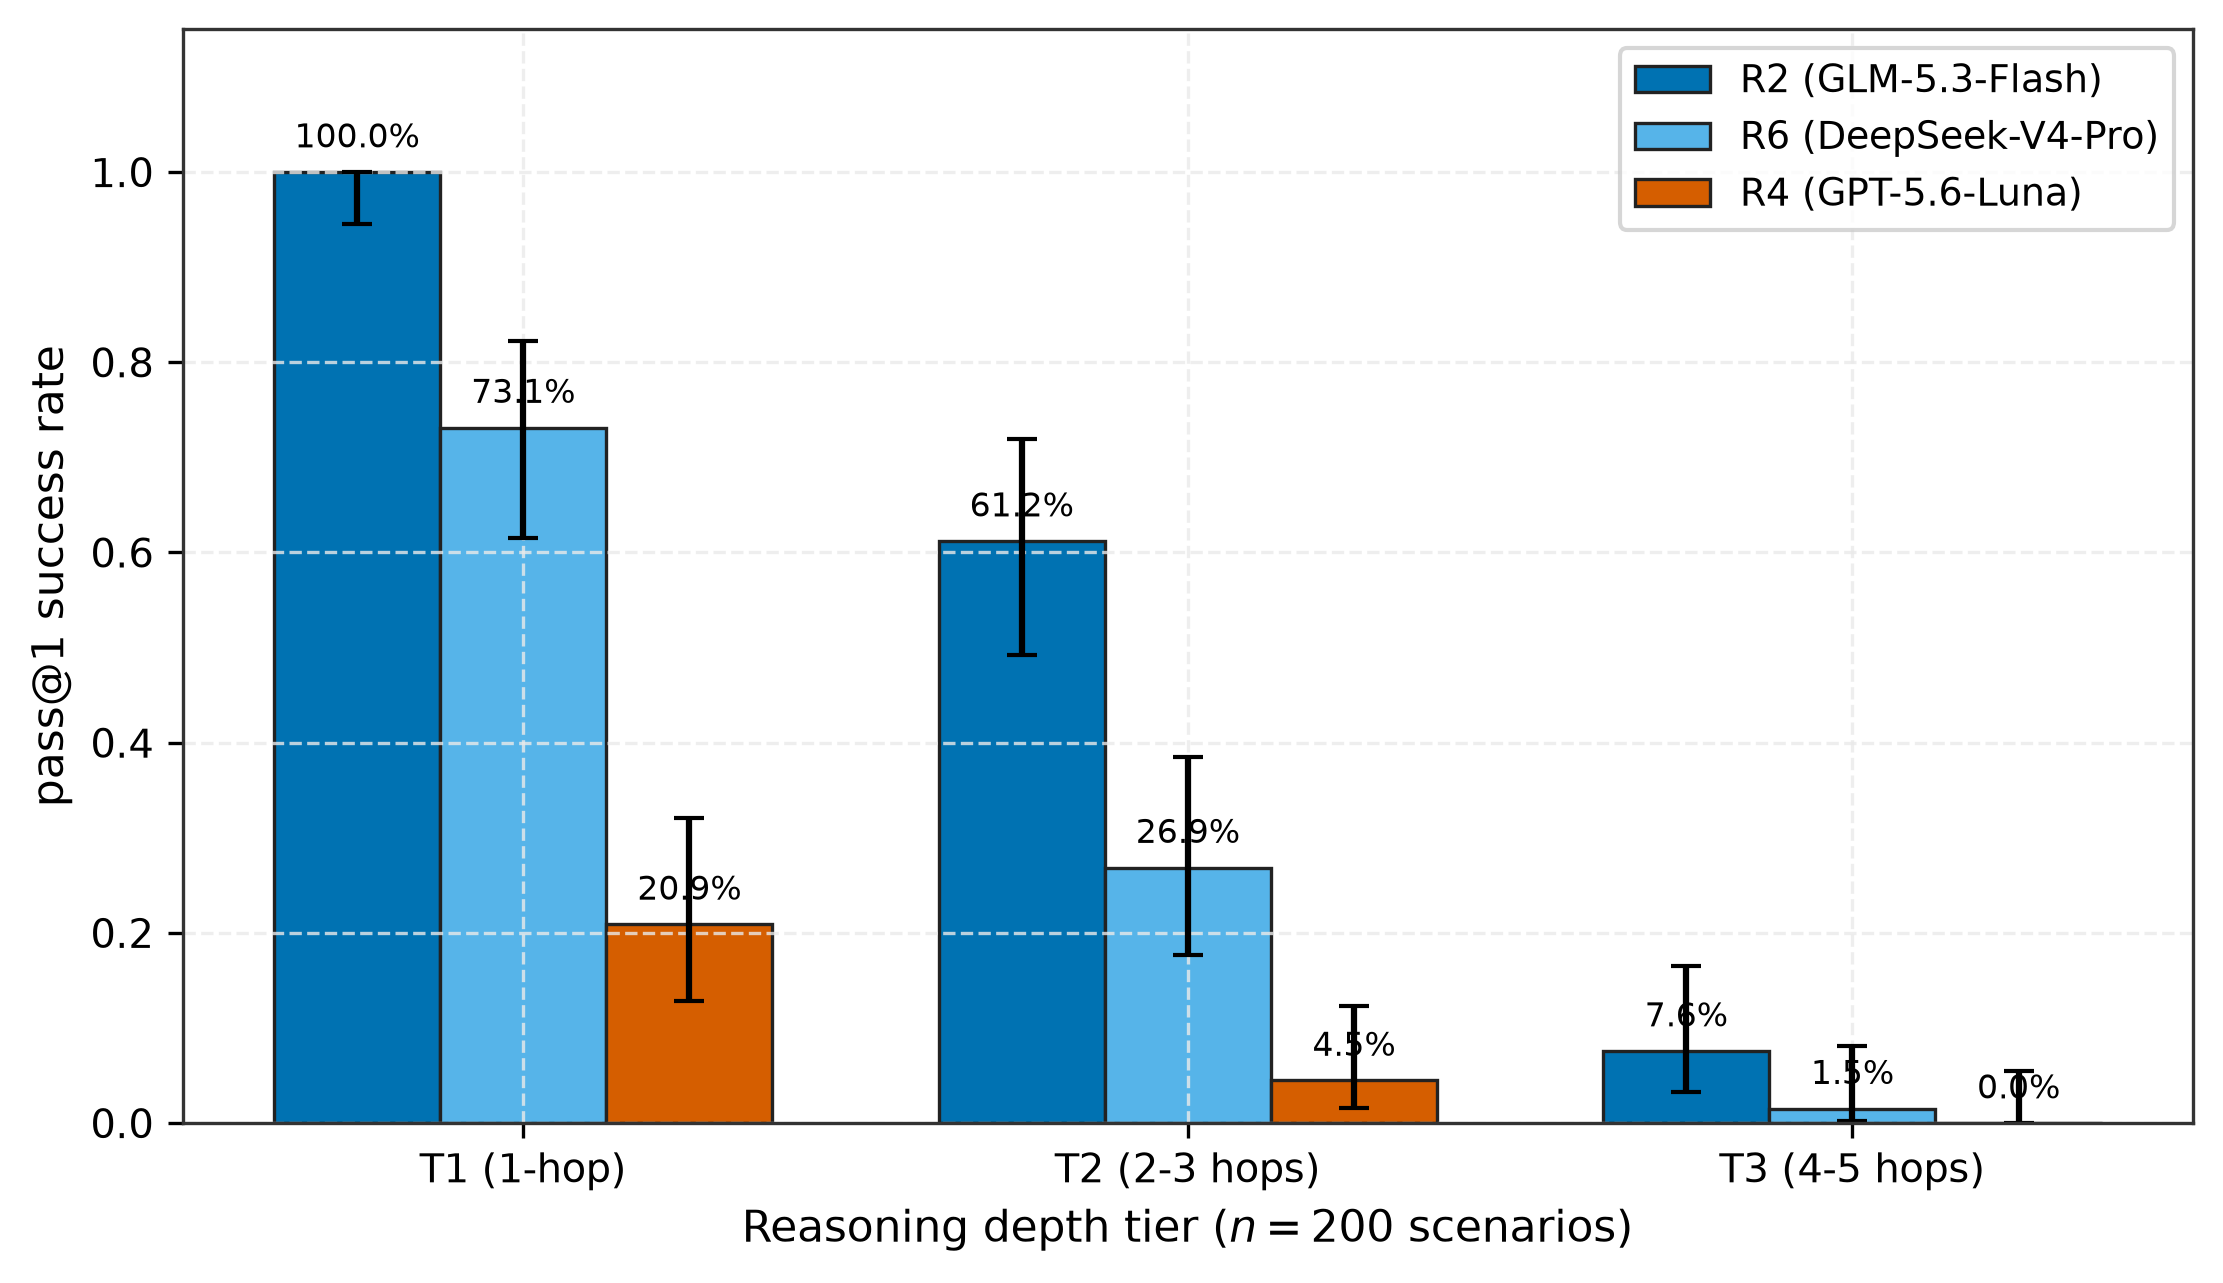
\includegraphics[width=0.85\textwidth]{fig_B_p03_depth.png}
\caption{Figure B: Single-trial pass@1 success rate across reasoning depth tiers (T1: 1-hop, $n=67$; T2: 2–3 hops, $n=67$; T3: 4–5 hops, $n=66$) for R2 (\texttt{glm-5.3-flash}), R6 (\texttt{deepseek-v4-pro}), and R4 (\texttt{gpt-5.6-luna}). Error bars represent 95\% Wilson score intervals.}
\label{fig:fig_B_p03_depth_png}
\end{figure}




\section*{Appendix C: P4 Failure Mode Taxonomy}
\addcontentsline{toc}{section}{Appendix C: P4 Failure Mode Taxonomy}

Qualitative axial coding of 200 execution traces from P3 (17 passing, 183 failing) was performed by the single author. Table C1 presents the failure mode taxonomy, raw counts, and prevalences (denominator = 183 failures).


\begin{table}[htbp]
\centering
\small
\setlength{\tabcolsep}{4.5pt}
\resizebox{\textwidth}{!}{
\begin{tabular}{lcccc}
\toprule
Failure Mode Identifier & Classification & Description & Count & Prevalence (\% of 183 failures) \\
\midrule
\texttt{INFRASTRUCTURE\_RATE\_LIMIT} & External Infrastructure & Remote HTTP 429 rate limit errors returned by cloud gateway & 114 & 62.30\% \\
\texttt{OVERCONSTRAINED\_SEARCH\_LOOP} & Emergent Agent Pathology & Agent generates overly specific search strings, entering repetitive query loops & 36 & 19.67\% \\
\texttt{MALFORMED\_TOOL\_CALL} & Agent Syntax Failure & Emitting invalid JSON or non-existent tool arguments & 23 & 12.57\% \\
\texttt{INFRASTRUCTURE\_SERVER\_ERROR} & External Infrastructure & Remote HTTP 500/502/503 server errors returned by gateway & 3 & 1.64\% \\
\texttt{MULTI\_HOP\_TRAVERSAL\_EXHAUSTION} & Emergent Agent Pathology & Valid multi-hop reasoning that hits the 12-step cap before reaching terminal target & 3 & 1.64\% \\
\texttt{RETRIEVAL\_FAILURE\_ABSTENTION} & Emergent Agent Pathology & Prematurely concluding target entity does not exist after initial search miss & 1 & 0.55\% \\
\texttt{ANSWER\_EXTRACTION\_TRUNCATION} & Emergent Agent Pathology & Correctly retrieving terminal document but truncating attribute in emitted answer & 1 & 0.55\% \\
\texttt{PREMATURE\_STOP\_WRONG\_HOP} & Emergent Agent Pathology & Terminating search at intermediate hop and outputting intermediate entity & 1 & 0.55\% \\
\texttt{MULTI\_HOP\_DIRECTION\_ERROR} & Emergent Agent Pathology & Traversing relational pointers in reverse direction from question prompt & 1 & 0.55\% \\
\bottomrule
\end{tabular}
}
\caption{Table C1: P4 human failure mode taxonomy. Five emergent modes absent from the baseline catalog confirmed hypothesis H2 [C038, C039, C040, C041, C042, C043, C044, C045, C046, C047, C048].}
\end{table}


Figure C illustrates the prevalence distribution across the nine axial failure modes.


\begin{figure}[htbp]
\centering
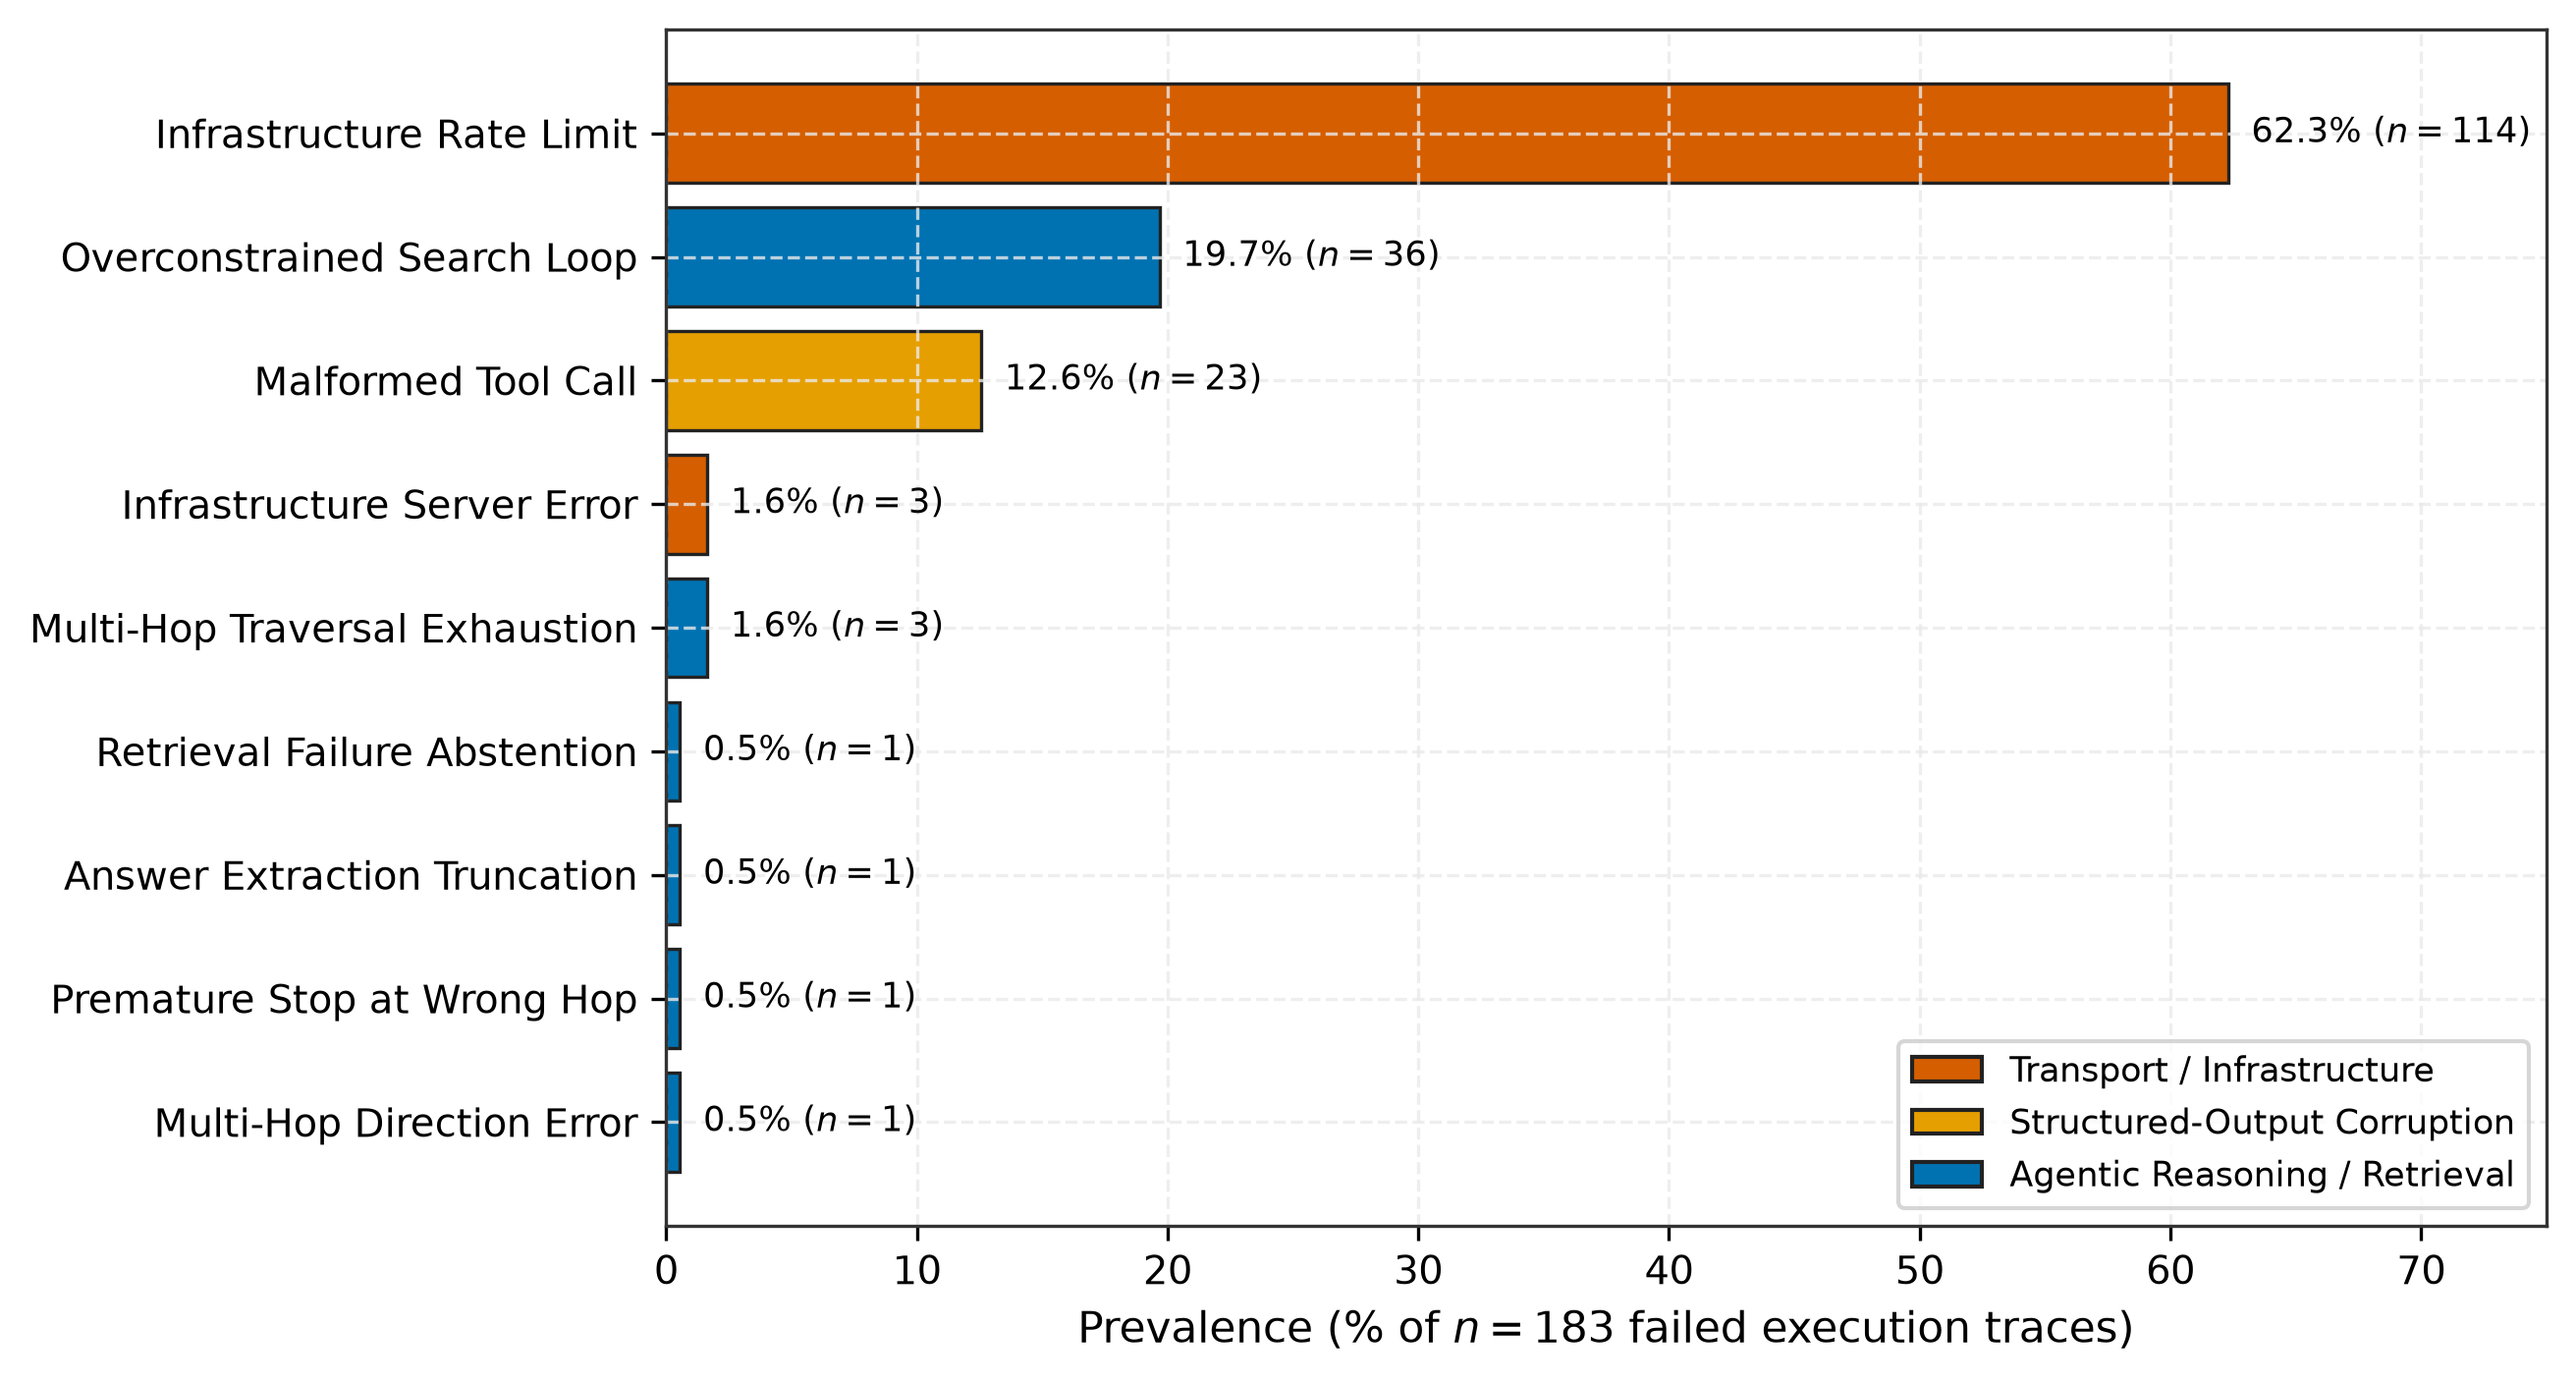
\includegraphics[width=0.85\textwidth]{fig_C_p04_taxonomy.png}
\caption{Figure C: Prevalence of 9 axial failure categories across $n=183$ failed execution traces in the P4 open/axial coding study. Transport infrastructure rate limits account for 62.3\% ($n=114$), overconstrained search loops for 19.7\% ($n=36$), and malformed tool calls for 12.6\% ($n=23$).}
\label{fig:fig_C_p04_taxonomy_png}
\end{figure}




\section*{Appendix D: P5 Evaluator Calibration and Degenerate Splits}
\addcontentsline{toc}{section}{Appendix D: P5 Evaluator Calibration and Degenerate Splits}

In P5, automated evaluators—deterministic code assertions and an LLM judge (\texttt{z-ai/glm-5.3})—were calibrated against human labels on a frozen $n=60$ test split. Table D1 summarizes evaluation performance, confusion matrices, chance-corrected agreement ($\kappa$), and Rogan-Gladen adjusted prevalence estimates [5, 13, 19].


\begin{table}[htbp]
\centering
\scriptsize
\setlength{\tabcolsep}{2.0pt}
\resizebox{\textwidth}{!}{
\begin{tabular}{lcccccccc}
\toprule
Evaluated Failure Mode & Evaluator Type & Confusion Matrix (TP, FP, TN, FN) & True Positive Rate (TPR) [95\% CI] & True Negative Rate (TNR) [95\% CI] & Cohen's $\kappa$ & Raw Prevalence & Rogan-Gladen Prevalence & Degenerate Split? \\
\midrule
\texttt{INFRASTRUCTURE\_RATE\_LIMIT} & Code Assertion & (34, 0, 26, 0) & 1.0000 [0.8985, 1.0000] & 1.0000 [0.8713, 1.0000] & 1.0000 & 0.5667 & 0.5667 & No \\
\texttt{OVERCONSTRAINED\_SEARCH\_LOOP} & LLM Judge & (0, 1, 45, 14) & 0.0000 [0.0000, 0.2153] & 0.9783 [0.8866, 0.9962] & -0.0321 & 0.2333 & 0.2333 & No \\
\texttt{MALFORMED\_TOOL\_CALL} & Code Assertion & (6, 21, 33, 0) & 1.0000 [0.6097, 1.0000] & 0.6111 [0.4779, 0.7296] & 0.2391 & 0.1000 & 0.1000 & No \\
\texttt{INFRASTRUCTURE\_SERVER\_ERROR} & Code Assertion & (1, 0, 59, 0) & 1.0000 [0.2065, 1.0000] & 1.0000 [0.9389, 1.0000] & 1.0000 & 0.0167 & 0.0167 & No \\
\texttt{MULTI\_HOP\_TRAVERSAL\_EXHAUSTION} & Code Assertion & (0, 7, 53, 0) & 1.0000 [0.0000, 1.0000] & 0.8833 [0.7782, 0.9423] & 0.0000 & 0.0000 & 0.0000 & \textbf{Yes ($\text{pos}=0$)} \\
\texttt{RETRIEVAL\_FAILURE\_ABSTENTION} & LLM Judge & (0, 0, 60, 0) & 1.0000 [0.0000, 1.0000] & 1.0000 [0.9398, 1.0000] & 1.0000 & 0.0000 & 0.0000 & \textbf{Yes ($\text{pos}=0$)} \\
\texttt{ANSWER\_EXTRACTION\_TRUNCATION} & LLM Judge & (0, 0, 60, 0) & 1.0000 [0.0000, 1.0000] & 1.0000 [0.9398, 1.0000] & 1.0000 & 0.0000 & 0.0000 & \textbf{Yes ($\text{pos}=0$)} \\
\texttt{PREMATURE\_STOP\_WRONG\_HOP} & LLM Judge & (0, 0, 59, 1) & 0.0000 [0.0000, 0.7935] & 1.0000 [0.9389, 1.0000] & 0.0000 & 0.0167 & 0.0000 & No \\
\texttt{MULTI\_HOP\_DIRECTION\_ERROR} & LLM Judge & (0, 0, 60, 0) & 1.0000 [0.0000, 1.0000] & 1.0000 [0.9398, 1.0000] & 1.0000 & 0.0000 & 0.0000 & \textbf{Yes ($\text{pos}=0$)} \\
\bottomrule
\end{tabular}
}
\caption{Table D1: P5 automated evaluator calibration against human labels ($n=60$). Modes with $\text{TP} + \text{FN} = 0$ represent degenerate test splits where metrics like $\kappa = 1.0$ reflect the absence of true positives rather than detection ability. [C049, C050, C051, C052, C053, C054, C055, C056, C057, C058, C059]}
\end{table}


Figure D plots the chance-corrected agreement ($\kappa$) across failure modes for the automated evaluators against human ground truth.


\begin{figure}[htbp]
\centering
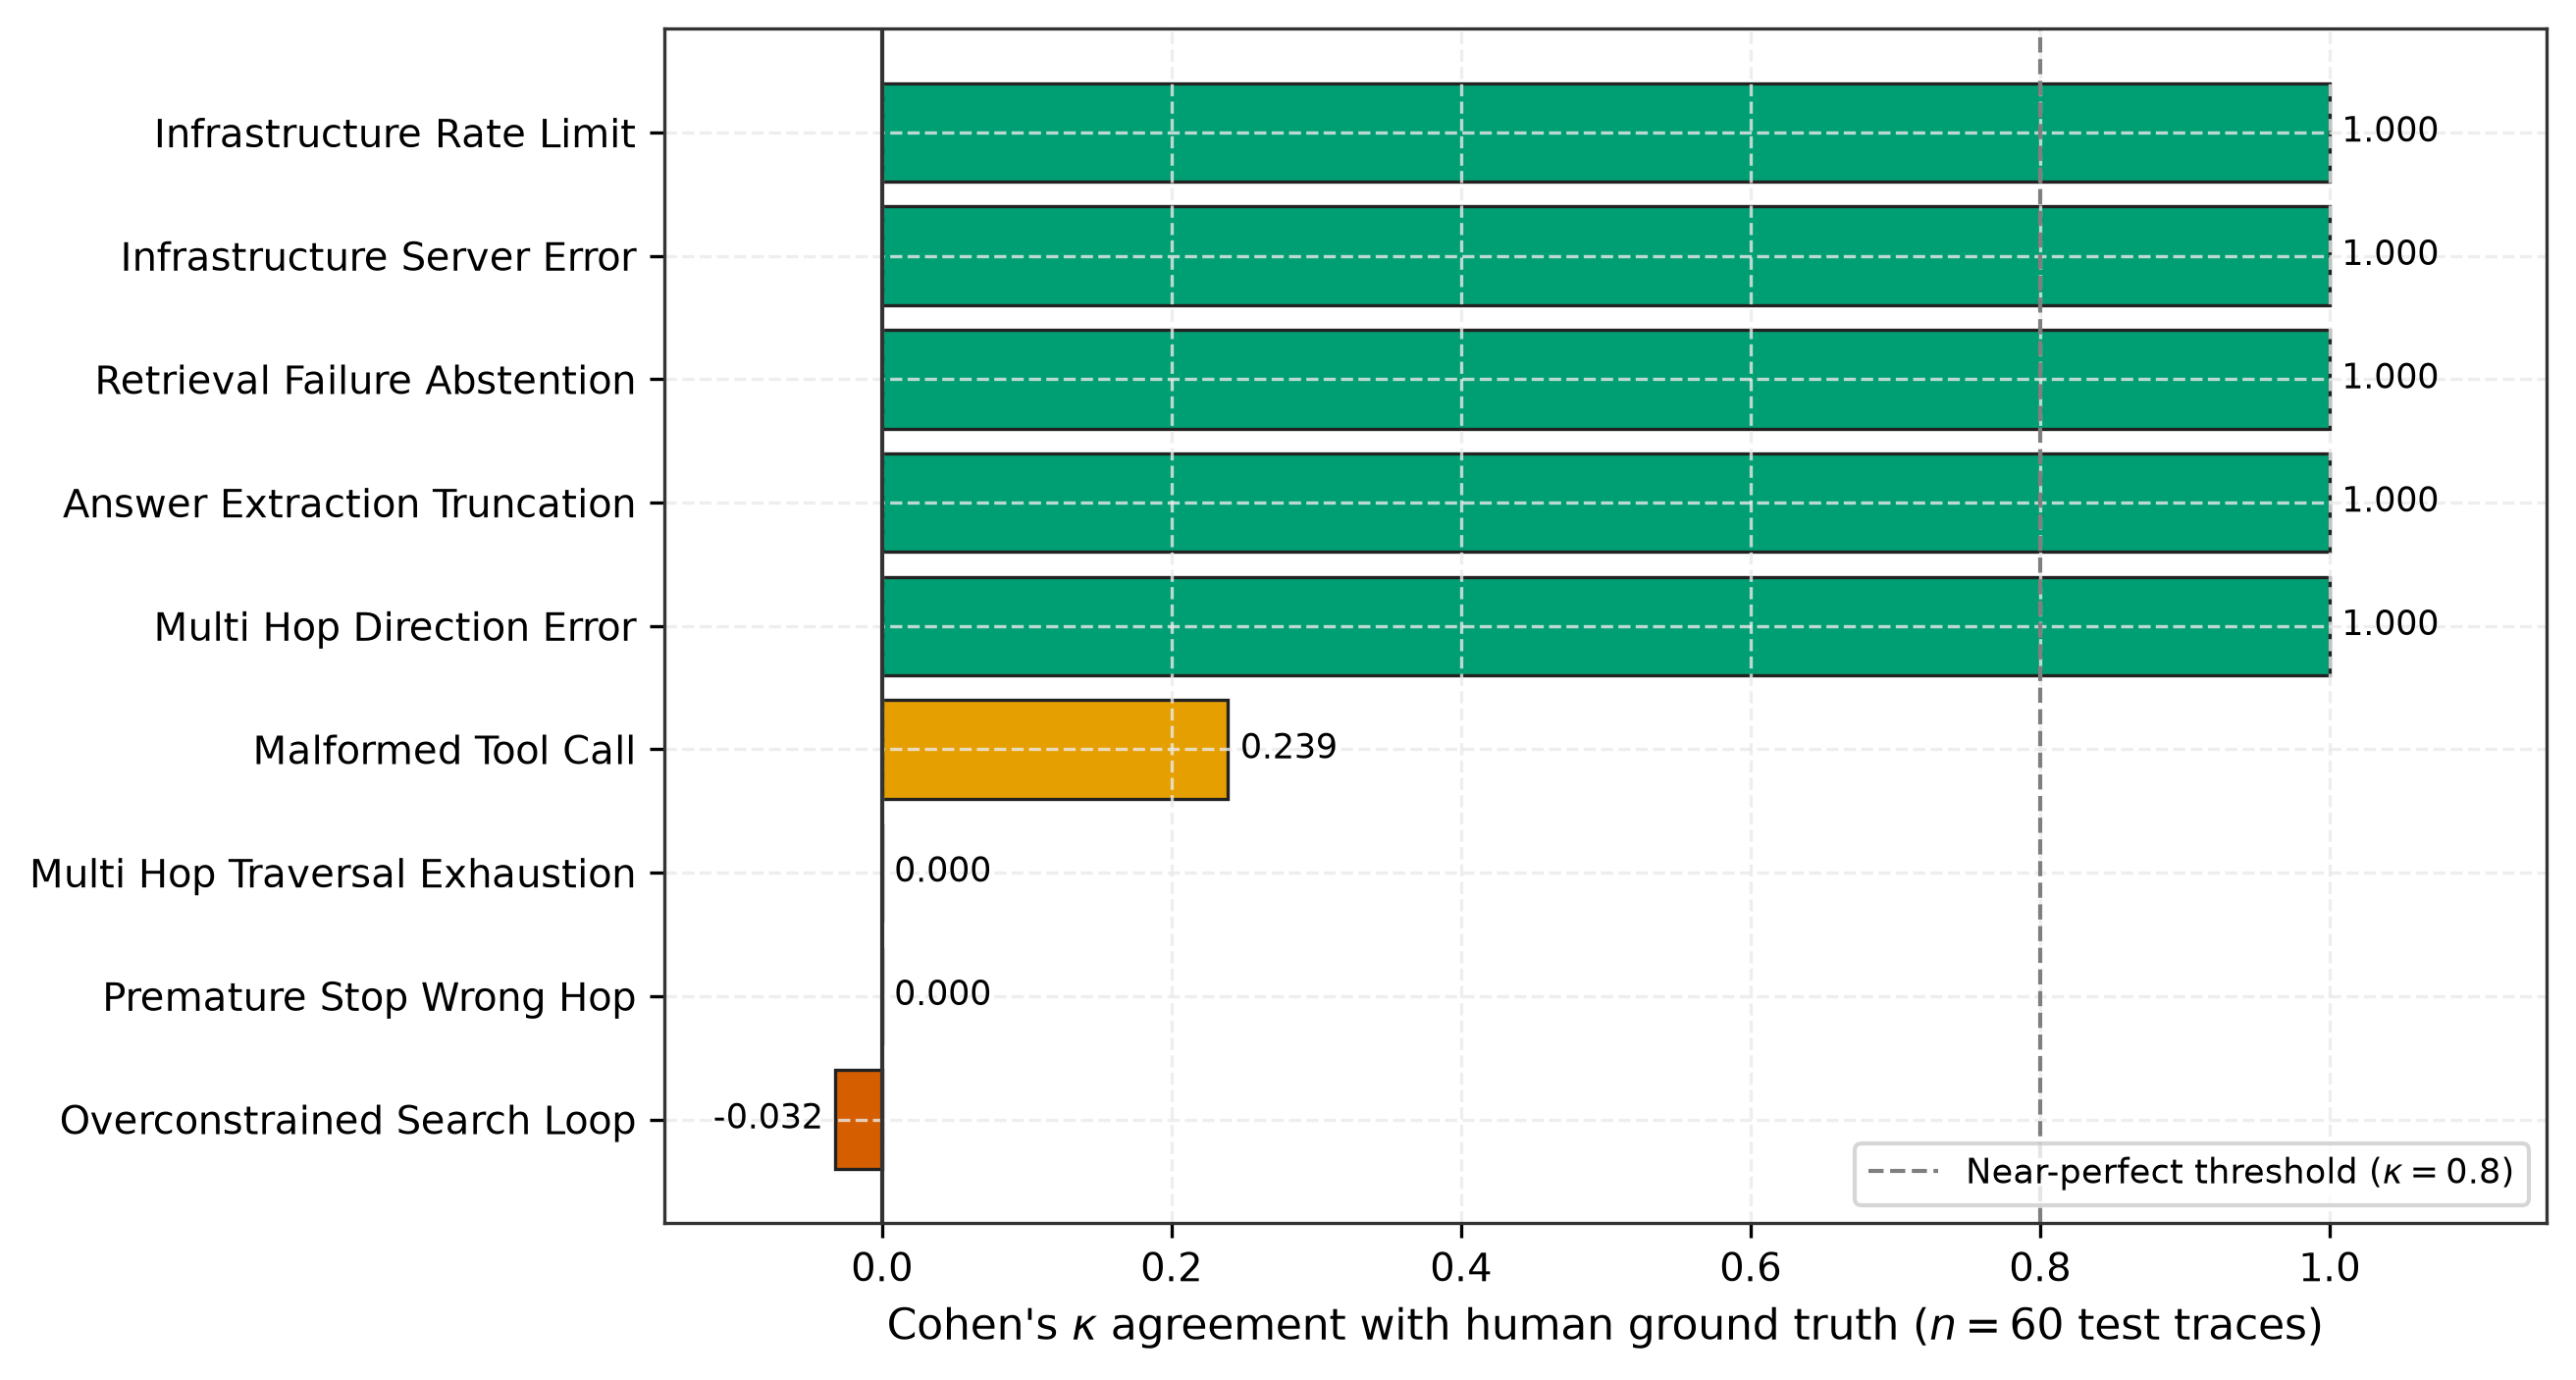
\includegraphics[width=0.85\textwidth]{fig_D_p05_kappa.png}
\caption{Figure D: Cohen's $\kappa$ inter-rater agreement for automated LLM evaluators against human axial ground truth on $n=60$ test traces across 9 failure modes. Five evaluators achieved perfect agreement ($\kappa = 1.0$), while multi-hop traversal exhaustion and premature stopping showed chance-level agreement ($\kappa = 0.0$) and search looping had negative agreement ($\kappa = -0.032$).}
\label{fig:fig_D_p05_kappa_png}
\end{figure}




\section*{Appendix E: Spend and Cost per Grounded Pass}
\addcontentsline{toc}{section}{Appendix E: Spend and Cost per Grounded Pass}

All API invocations were tracked via \texttt{ledger.jsonl}. Cumulative spend across the 900 primary runs in Pass 2 of Project P06 totaled \$23.0719 USD (\$5.0994 USD on R2, \$17.9725 USD on R4) across 35,401,507 tokens [C024, C067]. An earlier Pass 1 exploratory sweep (step cap 12) incurred \$0.3974 USD across 18,917,495 tokens (34.83\% of all generated tokens), bringing grand total project spend to \$23.4693 USD across 54,319,002 tokens [C024, C067]. Table E1 breaks down final-pass spend, passing trials, and cost per grounded pass.


\begin{table}[htbp]
\centering
\small
\setlength{\tabcolsep}{4.5pt}
\resizebox{\textwidth}{!}{
\begin{tabular}{lcccc}
\toprule
Model Tier \& Analysis & Final-Pass Spend (USD) & Passing Trials ($c$) & Cost per Grounded Pass (USD) [95\% Bootstrap CI] & Cost per Attempted Run (USD) \\
\midrule
\textbf{R2 (\texttt{z-ai/glm-5.3-flash}, as-run)} & \$5.0994 & 284 & \$0.017956 [\$0.016830, \$0.019316] & \$0.011332 \\
\textbf{R4 (\texttt{openai/gpt-5.6-luna}, as-run)} & \$17.9725 & 67 & \$0.268246 [\$0.213959, \$0.352402] & \$0.039939 \\
\textbf{R4 (\texttt{openai/gpt-5.6-luna}, infra-excluded)} & \$17.9725 & 67 & \$0.268246 [\$0.213959, \$0.352402] & \$0.051204 \\
\textbf{Pass 1 Discarded Sweep (R2 + R4)} & \$0.3974 & — & — & \$0.000442 \\
\textbf{Complete Study Cumulative} & \$23.4693 & 351 & — & \$0.017385 \\
\bottomrule
\end{tabular}
}
\caption{Table E1: Spend and cost per grounded pass across model tiers in Pass 2 and discarded Pass 1 sweep. Bootstrap intervals from 10,000 scenario-level resamples. [C024, C067]}
\end{table}




\section*{Appendix F: Anticipated Objections}
\addcontentsline{toc}{section}{Appendix F: Anticipated Objections}

We address seven anticipated methodological objections:

1. \textbf{"The benchmark relies entirely on a synthetic pseudoword graph rather than real-world tasks."}  
   \emph{Response:} Synthetic pseudoword graphs are intentionally employed to eliminate pre-training data contamination, ensuring agents cannot shortcut multi-hop reasoning via memorized semantic associations [2]. Every document link and attribute must be actively traversed via tool execution. However, [limitation] this paper cannot address whether failure clustering dynamics generalize to natural language documents with rich semantic redundancy.
2. \textbf{"Only two valid models were evaluated, precluding broad capability generalizations."}  
   \emph{Response:} We agree that evaluating two models (R2 and R4) cannot support broad generalizations across the ecosystem of LLM architectures. The third planned model (R6) suffered an irreversible external gateway collapse and was excluded from capability claims. Accordingly, we treat R2 and R4 strictly as empirical demonstrations of distinct accuracy regimes rather than a comprehensive model ranking [D-002, D-006].
3. \textbf{"The benchmark design favors one model architecture over another."}  
   \emph{Response:} All models received bitwise-identical system prompts, identical tool schema definitions, identical 24-step execution caps, and identical deterministic dual-condition oracle grading [C009, C014]. Neither prompt engineering nor tool tuning was performed to favor any provider. Differences in single-trial pass rates reflect intrinsic model tool-calling capability on 5-hop linear dependency chains.
4. \textbf{"The observed failure concentration is merely an empirical correlation, not an isolated causal mechanism."}  
   \emph{Response:} This objection is entirely correct. Our primary experiment establishes the statistical validity of the independence assumption on scenario-level outcomes; it does not isolate internal model attention dynamics. While our diagnostic studies (P3–P5) identify failure modes such as overconstrained search loops, [limitation] this paper cannot address causal mechanistic activations inside proprietary model weights.
5. \textbf{"The post-hoc exclusion of 33 infrastructure-contaminated scenarios undermines pre-registered rigor."}  
   \emph{Response:} To preserve methodological integrity, we report both the pre-registered as-run analysis ($n=150$) and the infra-excluded sensitivity analysis ($n=117$) side-by-side throughout the paper [D-008]. The 95 dropped trials exhibited a distinct latency signature ($<1$ ms fast-fails) following gateway timeouts, verifying an external failure mode. Disclosing both analyses demonstrates that while as-run data suggests strong failure concentration ($p=0.0123$), removing verifiable network dropouts renders the effect statistically marginal ($p=0.0488$) [C017, C028].
6. \textbf{"Why does joint reliability $\text{pass}^{3}$ matter if developers can simply retry failed tasks in production?"}  
   \emph{Response:} Retrying is only possible when an external verification oracle exists to detect failure immediately. In autonomous enterprise workflows (e.g., executing database transactions or clinical orders), agents operate unmonitored and benchmarks scoring single runs miss intermediate action-level divergence [1]. In these settings, joint reliability $\text{pass}^k$ represents the operational consistency requirement [12, 23].
7. \textbf{"Reproduction is impossible because closed commercial model API endpoints drift over time."}  
   \emph{Response:} Proprietary cloud API snapshot drift is an inherent challenge in contemporary empirical AI research [16, 18]. To maximize reproducibility, we have preserved the complete raw SQLite trace database containing all 1,350 execution traces, timestamps, latency signatures, and token counts (SHA256 \nolinkurl{1c83d147b5d7e5509a97eb46bf6fc400ca45b36aaa189bb18810bc75c56fe222}), enabling independent re-verification of all reported statistics without executing new API calls.
\end{document}
